%%%%%%%%%%%%%%%%%%%%%%%%%%%%%%%%%%%%%%%%%%
% Mathematics Final Year Research Projects
% LaTeX Template
% Version 1.0 (31/01/24)
%
% This template has been adapted from: https://www.overleaf.com/latex/templates/imperial-college-report-template/wncnzptkhnbc
% Students should feel free to adapt this template to their needs.
%%%%%%%%%%%%%%%%%%%%%%%%%%%%%%%%%%%%%%%%%%
%----------------------------------------------------------------------------------------
% PACKAGES AND OTHER DOCUMENT CONFIGURATIONS
%----------------------------------------------------------------------------------------
\documentclass[a4paper,11pt, twoside]{report}

%% Language and font encodings
\usepackage[english]{babel}
\usepackage[utf8]{inputenc}
\usepackage[T1]{fontenc}

%% Sets page size and margins
\usepackage[a4paper,top=1in,bottom=1in,left=1in,right=1in,marginparwidth=1.75cm]{geometry}

%% Useful packages
\usepackage{afterpage}
\usepackage{amsmath}
\usepackage{amsthm}
\usepackage{amssymb}
\usepackage{csquotes}
\usepackage{enumitem}
\usepackage{graphicx}
\usepackage{eurosym}
\usepackage{lipsum}
\usepackage{booktabs}
\usepackage{float}
\usepackage{indentfirst}
\usepackage{placeins}
% Listings (for displaying code):
\usepackage{listings}
\lstset{
    frame = single, 
    framexleftmargin=15pt
}

% Center figure captions:
\usepackage{caption}
\captionsetup[figure]{labelfont={bf},name={Figure},labelsep=quad}
\captionsetup[table]{labelfont={bf},name={Table},labelsep=quad}


% ----------- Algorithm2e setup
\usepackage[ruled,vlined]{algorithm2e}
\makeatletter
\renewcommand{\SetKwInOut}[2]{%
  \sbox\algocf@inoutbox{\KwSty{#2}\algocf@typo:}%
  \expandafter\ifx\csname InOutSizeDefined\endcsname\relax% if first time used
    \newcommand\InOutSizeDefined{}\setlength{\inoutsize}{\wd\algocf@inoutbox}%
    \sbox\algocf@inoutbox{\parbox[t]{\inoutsize}{\KwSty{#2}\algocf@typo:\hfill}~}\setlength{\inoutindent}{\wd\algocf@inoutbox}%
  \else% else keep the larger dimension
    \ifdim\wd\algocf@inoutbox>\inoutsize%
    \setlength{\inoutsize}{\wd\algocf@inoutbox}%
    \sbox\algocf@inoutbox{\parbox[t]{\inoutsize}{\KwSty{#2}\algocf@typo:\hfill}~}\setlength{\inoutindent}{\wd\algocf@inoutbox}%
    \fi%
  \fi% the dimension of the box is now defined.
  \algocf@newcommand{#1}[1]{%
    \ifthenelse{\boolean{algocf@inoutnumbered}}{\relax}{\everypar={\relax}}%
%     {\let\\\algocf@newinout\hangindent=\wd\algocf@inoutbox\hangafter=1\parbox[t]{\inoutsize}{\KwSty{#2}\algocf@typo\hfill:}~##1\par}%
    {\let\\\algocf@newinout\hangindent=\inoutindent\hangafter=1\parbox[t]{\inoutsize}{\KwSty{#2}\algocf@typo:\hfill}~##1\par}%
    \algocf@linesnumbered% reset the numbering of the lines
  }}%
\makeatother
% --------- end algorithm2e setup

% \bm allows typing bold math:
\usepackage{bm}
\usepackage[normalem]{ulem}

\usepackage[colorinlistoftodos]{todonotes}
\usepackage[colorlinks=true, allcolors=blue]{hyperref}

\renewcommand*{\rmdefault}{bch}
\renewcommand*{\ttdefault}{lmtt}
\newcommand{\citationneeded}{\textcolor{red}{[citation-needed]}}

\DeclareMathOperator*{\argmin}{\arg\!\min}
\DeclareMathOperator*{\argmax}{\arg\!\max}

% Add bigger skip between paragraphs, makes reading easier:
\setlength{\parskip}{0.5em}

% Bibliography
\usepackage[numbers, comma, square, sort&compress]{natbib}
\bibliographystyle{abbrvunsrtnat.bst}

%----------------------------------------------------------------------------------------
% END OF DOCUMENT CONFIGURATION
%----------------------------------------------------------------------------------------

%----------------------------------------------------------------------------------------
% IMPORTANT INFORMATION TO MODIFY FOR THE TITLE PAGE
%----------------------------------------------------------------------------------------
\newcommand{\reporttitle}{Behaviour-Based Money Mule Detection Using Supervised and Unsupervised Machine Learning} % Title of your research project
\newcommand{\reportauthor}{Baiqing Chen} % First Name and Last Name
\newcommand{\supervisor}{Nicola Gnecco} % First Name and Last Name of your supervisor(s)
\newcommand{\degreetype}{MSci in Mathematics} % MSci in Mathematics, BSc in Mathematics, BSc in Mathematics with Statistics, ...
%----------------------------------------------------------------------------------------
\raggedbottom
%----------------------------------------------------------------------------------------
% To compile this file, use the following sequence: 
%	latex main.tex
%	bibtex main.tex
%	latex main.tex
%	latex main.tex
%----------------------------------------------------------------------------------------

%----------------------------------------------------------------------------------------
% START OF DOCUMENT
%----------------------------------------------------------------------------------------
\begin{document}

% Title page
\begin{titlepage}

\newcommand{\HRule}{\rule{\linewidth}{0.5mm}} % Defines a new command for the horizontal lines, change thickness here


%----------------------------------------------------------------------------------------
%	LOGO SECTION
%----------------------------------------------------------------------------------------


\includegraphics[width=8cm]{title/logo.png}\\[1cm] % Include a department/university logo - this will require the graphicx package
 
%----------------------------------------------------------------------------------------

\center % Center everything on the page

%----------------------------------------------------------------------------------------
%	HEADING SECTIONS
%----------------------------------------------------------------------------------------

% For M3R or M4R reports, comment out as appropriate
\textsc{\LARGE Imperial College London}\\[0.5cm] % Name of your university/college
\textsc{\Large Department of Mathematics}\\[1.5cm] % Name of your department
\textsc{\Large MSci Research Project}\\[0.5cm] % Name of your programme
%\textsc{\LARGE BSc Research Project}\\[1.5cm] 

%----------------------------------------------------------------------------------------
%	TITLE SECTION
%----------------------------------------------------------------------------------------
\makeatletter
\HRule \\[0.6cm]
{ \huge \bfseries \reporttitle}\\[0.6cm] % Title of your document
\HRule \\[1.5cm]
 
%----------------------------------------------------------------------------------------
%	AUTHOR SECTION
%----------------------------------------------------------------------------------------

\begin{minipage}{0.4\textwidth}
\begin{flushleft} \large
\emph{Author:}\\
\reportauthor % Baiqing Chen
\end{flushleft}
\end{minipage}
~
\begin{minipage}{0.4\textwidth}
\begin{flushright} \large
\emph{Supervisor(s):} \\
\supervisor % Nicola Gnecco
\end{flushright}
\end{minipage}\\[2cm]
\makeatother

%----------------------------------------------------------------------------------------
%	FOOTER & DATE SECTION
%----------------------------------------------------------------------------------------
\vfill % Fill the rest of the page with whitespace
Submitted in partial fulfillment of the requirements for the \degreetype~at Imperial College London\\[0.5cm]

\makeatletter
{\large \today}\\[2cm] % Date, change the \today to a set date if you want to be precise
\makeatother

\end{titlepage}

% Abstract
\begin{abstract}

Money mule accounts play a central role in money laundering by transferring illicit funds through legitimate banking systems. Detecting such accounts is challenging because labelled examples are scarce and mule behaviour often resembles normal customer activity.

This project investigates whether behavioural features engineered from transaction histories can improve money mule detection. A range of account-level features describing transaction activity, pass-through behaviour and fund movement patterns were constructed from retail banking transaction data. Both unsupervised methods, including DBSCAN clustering and autoencoder-based anomaly detection, and supervised classifiers, including Logistic Regression and XGBoost, were evaluated.

The results show that behavioural feature engineering provides useful information for distinguishing potentially suspicious accounts. The supervised models achieved stronger predictive performance when confirmed labels were available, while the unsupervised approaches were able to identify anomalous behavioural patterns without requiring labelled data. The study also highlights practical challenges, including limited labelled data and the computational cost of certain behavioural features.

Overall, the findings demonstrate that behavioural transaction features provide an effective basis for money mule detection and offer insights into the strengths and limitations of supervised and unsupervised machine learning approaches in anti-money laundering applications.

\end{abstract}
 
% Acknowledgements
\clearpage
\section*{Acknowledgments}


I would like to express my gratitude to my supervisor, Nicola Gnecco, for his guidance, support, and feedback throughout this project.

My thanks also go to Joao Fernandes and Pedro Jorge at Novo Banco for their valuable guidance, practical advice, and support during the development of this work. Their insights helped me better understand the data, the business context, and the challenges involved in money mule detection.

I would also like to thank my parents and friends for their constant encouragement and emotional support. Without their patience, understanding, and belief in me, I would not have been able to complete this thesis.

Finally, I would like to thank myself for persevering through the difficulties, uncertainty, and pressure of this project, and for continuing to move forward until the end.

\clearpage

% Acknowledgements
\clearpage
\section*{Plagiarism statement}
The work contained in this thesis is my own work unless otherwise stated. Generative AI tools, including ChatGPT and GitHub Copilot, were used to support code development and language editing. All final content, analysis, interpretations, and conclusions remain my own.\\

\vspace{1em}
\noindent \textit{Signature:} \reportauthor \\
\textit{Date:} \today
\clearpage

% Table of contents
\tableofcontents

% Main sections of the report
% ===========================
% Uncomment or add folders to add your own chapters and input files.

\chapter{Introduction}

Financial institutions process large volumes of customer transactions every day. While most of these transactions reflect legitimate economic activity, a small proportion may be associated with financial crime. One important example is the use of money mule accounts. Money mules are individuals or entities whose accounts are used to receive and transfer illicit funds on behalf of criminal networks. These accounts may be opened deliberately for criminal purposes, but they may also belong to individuals who have been recruited, deceived, or coerced into moving money. Detecting such accounts is therefore an important component of anti-money laundering and fraud prevention systems.

Money mule detection is challenging for several reasons. First, mule accounts are rare relative to the overall customer population, creating a highly imbalanced detection problem. Second, mule behaviour may not be captured by a single transaction or a single account-level statistic. Instead, suspicious behaviour often arises from combinations of transaction patterns, such as incoming funds being rapidly forwarded onwards, one incoming transfer being followed by multiple outgoing payments, or unusually high outgoing intensity shortly after receipt of funds. Third, many legitimate customers may display superficially similar behaviour. For example, active retail customers may make frequent outgoing payments, receive salary or family transfers, or spend incoming funds over time. This makes it difficult to distinguish mule-like behaviour from normal customer activity using simple rules alone.

This project investigates whether account-level behavioural features can be used to identify customer accounts with mule-like transaction patterns. The analysis was conducted using bank transaction data aggregated at the party level, so that each observation represents the behaviour of one customer rather than one individual transaction. This choice reflects the practical objective of identifying suspicious customer accounts for further review. A set of behavioural features was engineered to describe transaction activity, outgoing intensity, pass-through behaviour, one-in-many-out patterns, draining behaviour, and activity timing. These features were designed to capture both general account activity and more specific mule-related behaviours.

The modelling strategy combines unsupervised and supervised approaches. DBSCAN was used as the main unsupervised clustering method to segment customer behaviour and identify observations that do not belong to dense regions of normal retail activity. An autoencoder was also used as an unsupervised reconstruction-based anomaly detection model, where accounts with large reconstruction errors were interpreted as more unusual relative to the training distribution. These unsupervised methods are useful because confirmed mule labels are limited and the majority of accounts are unlabeled.

In addition, a small set of confirmed mule accounts was used to construct supervised baseline models. Logistic regression was used as an interpretable linear baseline, while XGBoost was used as a more flexible non-linear tree-based model capable of capturing interactions between behavioural features. Since confirmed mule accounts formed only a small minority of the modelling dataset, class weighting was applied to reduce the tendency of supervised models to favour the majority unlabeled class. The supervised model outputs were interpreted as relative mule-risk scores rather than calibrated probabilities, because the confirmed mule accounts were appended to a sampled retail comparison group and the unlabeled class may contain hidden mule accounts.

The main objective of this thesis is to develop and evaluate a behavioural detection framework for identifying mule-like accounts in bank transaction data. The project combines customer-level feature engineering with both unsupervised anomaly detection and supervised classification models, so that suspicious accounts can be segmented, scored, and ranked according to mule-risk. In particular, the thesis compares DBSCAN and autoencoder-based anomaly detection with logistic regression and XGBoost supervised baselines, evaluates the extent to which engineered behavioural features improve detection, and analyses which transaction patterns drive the resulting risk scores under a partially labelled setting.

The remainder of this thesis is organised as follows. Chapter 2 provides background on money mule behaviour, anomaly detection, and supervised learning methods relevant to financial crime detection. Chapter 3 describes the data and preprocessing steps. Chapter 4 presents the feature engineering process, including activity-based features and mule-behaviour features. Chapter 5 describes the modelling methodology, including DBSCAN, the autoencoder, logistic regression, and XGBoost. Chapter 6 presents and interprets the experimental results. Finally, Chapter 7 discusses the limitations of the study and outlines possible directions for future work.





\chapter{Background}
Money mule accounts play a critical role in modern financial crime schemes, including fraud, money laundering, and the movement of illicit funds. A money mule is an individual or entity that transfers or receives money on behalf of criminals, often allowing illegal funds to pass through seemingly legitimate bank accounts before being withdrawn, transferred, or dispersed to other destinations (\cite{homeoffice2024moneymule}). The increasing use of digital banking channels, instant payments, and cross-border transactions has made the identification of money mule activity an important challenge for financial institutions and regulatory authorities.The scale of fraud-related losses illustrates the importance of this challenge. According to Annual Fraud Report 2025 \cite{ukfinance2025annualfraud}, in the UK,
reported fraud losses across authorised and unauthorised channels reached approximately
\pounds1.17 billion in 2024, with 3.31 million confirmed cases. Authorised push payment
(APP) fraud alone accounted for around \pounds450.7 million of losses, and Faster Payments
were used in 96\% of fraudulent APP scam payments. Since mule accounts are commonly used
to receive and move the proceeds of such fraud, these figures highlight the importance of
detecting suspicious receiving and onward-transfer behaviour in modern payment systems.

The presence of money mule accounts poses significant risks to the financial system. These accounts facilitate the laundering of proceeds from fraud, cybercrime, and other criminal activities, making it more difficult for authorities to trace the origin and destination of illicit funds. Beyond direct financial losses, money mule networks contribute to reputational damage, regulatory penalties, increased compliance costs, and reduced trust in financial institutions. Consequently, the early detection of money mule behaviour has become a key objective within anti-money laundering (AML) and fraud prevention frameworks.The operational scale of mule networks is reflected in recent law-enforcement activity. Europol's
European Money Mule Action 2023 \cite{europol2023papertrail} identified 10,759 money mules and 474 recruiters or herders,
leading to 1,013 arrests and 4,659 investigations, with approximately \euro32 million in
prevented losses. Similarly, the US Department of Justice reported enforcement actions against
more than 3,000 money mules in its 2024 Money Mule Initiative \cite{doj2024moneymules}. These figures suggest that
money mule activity is not limited to isolated suspicious accounts, but often forms part of
larger organised networks.

Detecting money mule accounts is challenging for several reasons. First, genuine mule accounts often resemble legitimate customers in terms of account ownership, customer demographics, and transaction volumes. Second, mule behaviour is highly heterogeneous and may manifest through multiple transaction patterns. For example, some mule accounts exhibit rapid cash-out behaviour, where incoming funds are quickly withdrawn or transferred shortly after receipt. Others act as pass-through accounts, receiving funds from multiple sources before redistributing them to multiple destinations. Furthermore, new laundering strategies continuously emerge, making it difficult to rely solely on predefined rules or known typologies.

Empirical evidence from known mule accounts supports the importance of these behavioural
signals. A RUSI study \cite{westmore2025followingfraud} using data provided by Lloyds Bank analysed \pounds7.2 million of
outbound transactions from known money mule accounts between June and August 2024. The
study found that nearly 28\% of incoming value left mule accounts within 15 minutes, a further
25\% left within one hour, and less than 15\% remained after 24 hours. It also found that 57\%
of outbound value left via Faster Payments, while debit card spending, inter-account transfers
and cash withdrawals accounted for 18\%, 11\% and 10\%, respectively. These findings motivate
the construction of features capturing pass-through behaviour, short-window outflows,
transaction velocity, and fan-out patterns.

Traditional rule-based monitoring systems remain widely used in financial institutions. While such systems can effectively identify known suspicious patterns, they often generate large numbers of false positives and may struggle to detect previously unseen behaviours. Machine learning approaches provide an alternative by analysing large volumes of transaction data and identifying unusual behavioural patterns automatically. In particular, unsupervised anomaly detection techniques are attractive because labelled examples of confirmed money mule accounts are often scarce, incomplete, or unavailable.

This thesis investigates the detection of potential money mule accounts using large-scale banking transaction data. The study focuses on modelling account-level transactional behaviour through the construction of behavioural features derived from account activity, transaction flows, and payment characteristics. By analysing patterns of fund movement and identifying accounts whose behaviour deviates from typical customer activity, the objective is to develop a framework capable of prioritising potentially suspicious accounts for further investigation.

\chapter{Data Preprocessing}
The dataset consists of retail banking transaction records provided by Novo Banco. Information is distributed across multiple relational tables, including customer identifiers, financial contracts, instruments, and transaction records. Transactions contain information such as booking timestamp, transaction amount, transaction type, and transaction channel .All personal data has been anonymised.

The original data structure is transaction-level, where each row represents a single financial transaction associated with a customer account. Since the objective of this project is to identify suspicious customers rather than suspicious individual transactions, the data were transformed into a customer-level representation.

To capture the overall behaviour of a customer across multiple banking products and accounts, transactions were aggregated at the customer level. A party may be linked to multiple financial contracts and instruments, allowing all activity associated with the same customer to be analysed jointly.

Following aggregation, each row in the modelling dataset corresponds to a single customer, represented by a set of behavioural features derived from the customer's transaction history.
\chapter{Feature Engineering}

This chapter describes the construction of account-level behavioural features used for money mule detection. Since the raw data are recorded at transaction level, features were aggregated at the party level, so that each observation in the modelling dataset corresponds to one customer.

Let \(i\) denote a party and let \(\mathcal{T}_i\) be the set of transactions associated with party \(i\). Each transaction \(j \in \mathcal{T}_i\) has an amount \(x_{ij}\), a booking time \(t_{ij}\), and a direction \(d_{ij} \in \{\mathrm{IN}, \mathrm{OUT}\}\).

\section{Basic Activity Features}

Basic activity features were constructed to describe the overall transaction profile of each party, including transaction frequency, monetary volume, and temporal activity.

The total number of transactions for party \(i\) is defined as
\[
N_i = |\mathcal{T}_i|.
\]
The number of incoming and outgoing transactions are given by
\[
N_i^{in} = \sum_{j \in \mathcal{T}_i} \mathbf{1}(d_{ij}=\mathrm{IN}),
\qquad
N_i^{out} = \sum_{j \in \mathcal{T}_i} \mathbf{1}(d_{ij}=\mathrm{OUT}).
\]
Similarly, the total incoming and outgoing amounts are defined as
\[
A_i^{in} = \sum_{j \in \mathcal{T}_i: d_{ij}=\mathrm{IN}} x_{ij},
\qquad
A_i^{out} = \sum_{j \in \mathcal{T}_i: d_{ij}=\mathrm{OUT}} x_{ij}.
\]

To account for differences in account activity duration, activity-based normalisation was applied. Let \(D_i^{span}\) denote the number of days between the first and last observed transaction for party \(i\), and let \(D_i^{active}\) denote the number of distinct days on which party \(i\) made at least one transaction. Transaction intensity was then measured by
\[
V_i^{span} = \frac{N_i}{\max(D_i^{span},1)},
\qquad
V_i^{active} = \frac{N_i}{\max(D_i^{active},1)}.
\]

Temporal activity features were also included. The off-hours ratio and weekend ratio were defined as
\[
R_i^{off} =
\frac{N_i^{off}}{\max(N_i,1)},
\qquad
R_i^{weekend} =
\frac{N_i^{weekend}}{\max(N_i,1)}.
\]
These features capture whether a customer tends to transact outside standard daytime hours or during weekends.

\section{Amount-Based Transformation Features}

Transaction amounts are typically highly right-skewed, with a small number of very large transactions. To reduce the influence of extreme values, logarithmic transformations were applied to selected amount-based variables:
\[
x^{log} = \log(1+x).
\]
For example, daily incoming and outgoing monetary volumes were transformed as
\[
L_i^{in} =
\log\left(1 + \frac{A_i^{in}}{\max(D_i^{span},1)}\right),
\qquad
L_i^{out} =
\log\left(1 + \frac{A_i^{out}}{\max(D_i^{span},1)}\right).
\]

Additional amount distribution features were constructed to describe the shape of each customer's transaction amount distribution. Let \(m_i\) denote the median transaction amount for party \(i\), \(\bar{x}_i\) the mean transaction amount, \(P_{90,i}\) the 90th percentile, and \(x_{i}^{max}\) the maximum transaction amount. The following features were computed:
\[
G_i = \bar{x}_i - m_i,
\]
\[
G_i^{rel} =
\frac{\bar{x}_i - m_i}{\max(\bar{x}_i,1)},
\]
\[
Q_i^{90/50} =
\frac{P_{90,i}}{\max(m_i,1)},
\qquad
Q_i^{max/50} =
\frac{x_i^{max}}{\max(m_i,1)}.
\]
These features capture whether an account is characterised by occasional unusually large transactions relative to its typical transaction size.

\section{Ratio Features}

Several ratio features were constructed to describe the balance between incoming and outgoing activity. The outgoing transaction ratio and incoming transaction ratio are defined as
\[
R_i^{out,txn} =
\frac{N_i^{out}}{\max(N_i^{in}+N_i^{out},1)},
\qquad
R_i^{in,txn} =
\frac{N_i^{in}}{\max(N_i^{in}+N_i^{out},1)}.
\]
The outgoing amount ratio was defined as
\[
R_i^{out,amt} =
\frac{A_i^{out}}{\max(A_i^{in}+A_i^{out},1)}.
\]
These ratios help distinguish accounts dominated by incoming activity, outgoing activity, or balanced fund movement.

\section{Money Mule Behaviour Features}

Money mule accounts are often characterised by rapid fund forwarding: funds are received and then transferred out shortly afterwards. To capture this behaviour, features were constructed using forward-looking time windows after each incoming transaction. In the final implementation, one-hour and twenty-four-hour windows were retained.

Let \(k\) denote an incoming transaction of party \(i\), with amount \(a_{ik}\) and timestamp \(t_{ik}\). For a time window \(w \in \{1h,24h\}\), define the outgoing amount following this incoming transaction as
\[
O_{ik}^{(w)}
=
\sum_{\substack{j \in \mathcal{T}_i:\\
d_{ij}=\mathrm{OUT},\;
t_{ik}<t_{ij}\leq t_{ik}+w}}
x_{ij}.
\]

\subsection{Near Pass-Through Features}

The pass-through ratio for incoming transaction \(k\) is defined as
\[
P_{ik}^{(w)}
=
\frac{O_{ik}^{(w)}}{\max(a_{ik},1)}.
\]
A near pass-through event is recorded when the outgoing amount is close to the incoming amount:
\[
I_{ik}^{pass,(w)}
=
\mathbf{1}\left(a \leq P_{ik}^{(w)} \leq b\right).
\]
Where a and b are two real number thresholds. The party-level near pass-through ratio is then
\[
R_i^{pass,(w)}
=
\frac{1}{\max(N_i^{in},1)}
\sum_{k=1}^{N_i^{in}}
I_{ik}^{pass,(w)}.
\]
This feature measures the proportion of incoming transactions that are followed by a near-equivalent outflow within the specified time window.

\subsection{One-In-Many-Out Features}

Money mule accounts may also disperse funds through multiple outgoing payments after receiving an incoming transfer. Let
\[
C_{ik}^{out,(w)}
=
\sum_{\substack{j \in \mathcal{T}_i:\\
d_{ij}=\mathrm{OUT},\;
t_{ik}<t_{ij}\leq t_{ik}+w}}
1
\]
be the number of outgoing transactions following incoming transaction \(k\) within window \(w\). A one-in-many-out event is defined as
\[
I_{ik}^{many,(w)}
=
\mathbf{1}\left(C_{ik}^{out,(w)} \geq n\right).
\]
Where n is a threshold. The corresponding party-level ratio is
\[
R_i^{many,(w)}
=
\frac{1}{\max(N_i^{in},1)}
\sum_{k=1}^{N_i^{in}}
I_{ik}^{many,(w)}.
\]
This feature approximates fan-out behaviour, where a single incoming payment is followed by several outgoing payments.

\subsection{Outgoing Intensity and Method Diversity}

In addition to the ratio features, the maximum number of outgoing transactions following any incoming transaction was recorded:
\[
M_i^{out,(w)}
=
\max_k C_{ik}^{out,(w)}.
\]
This captures the most intense observed fund dispersion event for each party.

For the one-hour window, outgoing method diversity was also computed as the number of distinct outgoing transaction types following an incoming transaction:
\[
D_{ik}^{method,(1h)}
=
\left|
\left\{
\mathrm{type}_{ij}:
d_{ij}=\mathrm{OUT},
\;
t_{ik}<t_{ij}\leq t_{ik}+1h
\right\}
\right|.
\]
The maximum method diversity across incoming anchors was then used as a party-level feature:
\[
D_i^{method}
=
\max_k D_{ik}^{method,(1h)}.
\]

Counterparty information was not included in the current implementation due to computational constraints. Therefore, fan-out behaviour is approximated using the number of outgoing transactions rather than the number of distinct beneficiaries.
\subsection{Drain Ratio}

The near pass-through features described above are count-based: they measure the proportion of incoming transactions that are followed by approximately equivalent outgoing transfers. However, this may lose information about monetary importance. For example, several small incoming transactions may dominate the count-based ratio, while a single large incoming transfer that is rapidly drained may have greater relevance from a money mule detection perspective.

To incorporate the monetary scale of the behaviour, a drain ratio feature was constructed. For each incoming transaction \(k\) of party \(i\), with amount \(a_{ik}\), outgoing transactions occurring within a predefined window \(w\) (1h/24h) after the incoming transaction are considered. Outgoing amounts are allocated using a First-In-First-Out (FIFO) matching procedure, so that each outgoing amount is assigned to the earliest eligible incoming transaction and cannot be counted multiple times.

Let \(D_{ik}^{(w)}\) denote the amount of incoming transaction \(k\) that is drained through outgoing transfers within window \(w\). The party-level drain ratio is then defined as
\[
R_i^{\mathrm{drain},(w)}
=
\frac{\sum_{k=1}^{N_i^{in}} D_{ik}^{(w)}}
{\sum_{k=1}^{N_i^{in}} a_{ik}}.
\]

This feature measures the proportion of the total inbound monetary volume over the customer's observed transaction history that is transferred out within a short period of receipt. Unlike the near pass-through ratio, it is amount-weighted and does not require the outgoing amount to be close to the incoming amount for each individual transaction.

\begin{figure}[ht]
    \centering
    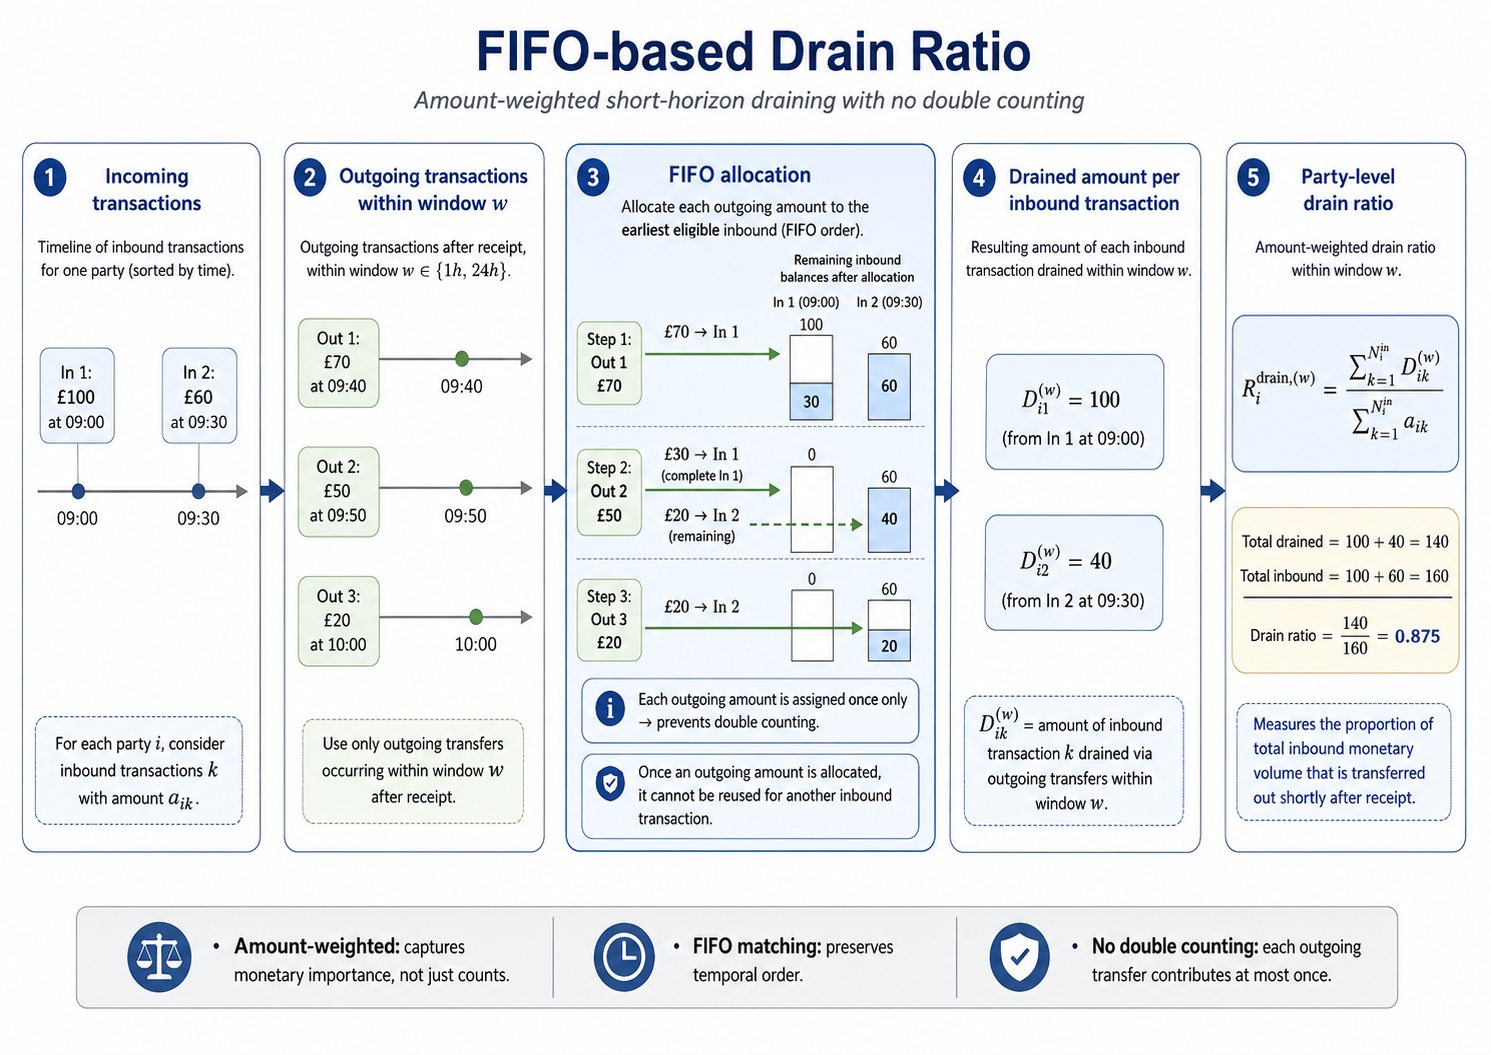
\includegraphics[width=0.55\textwidth]{methods/ChatGPT Image 2026年6月20日 13_20_06.png}
    \caption{FIFO drain diagram}
    \label{fig:autoencoder_architecture}
\end{figure}
\chapter{Methods}
\section{DBSCAN}
Density-Based Spatial Clustering of Applications with Noise (DBSCAN) was used as the main unsupervised clustering method \cite{ester1996density}. DBSCAN is suitable for this problem because it does not require the number of clusters to be specified in advance and explicitly identifies observations that do not belong to any dense region as noise. This is useful in the context of money mule detection, where suspicious accounts are expected to form a small minority of the population and may not constitute a well-separated spherical cluster.  
\begin{figure} 
    \centering
    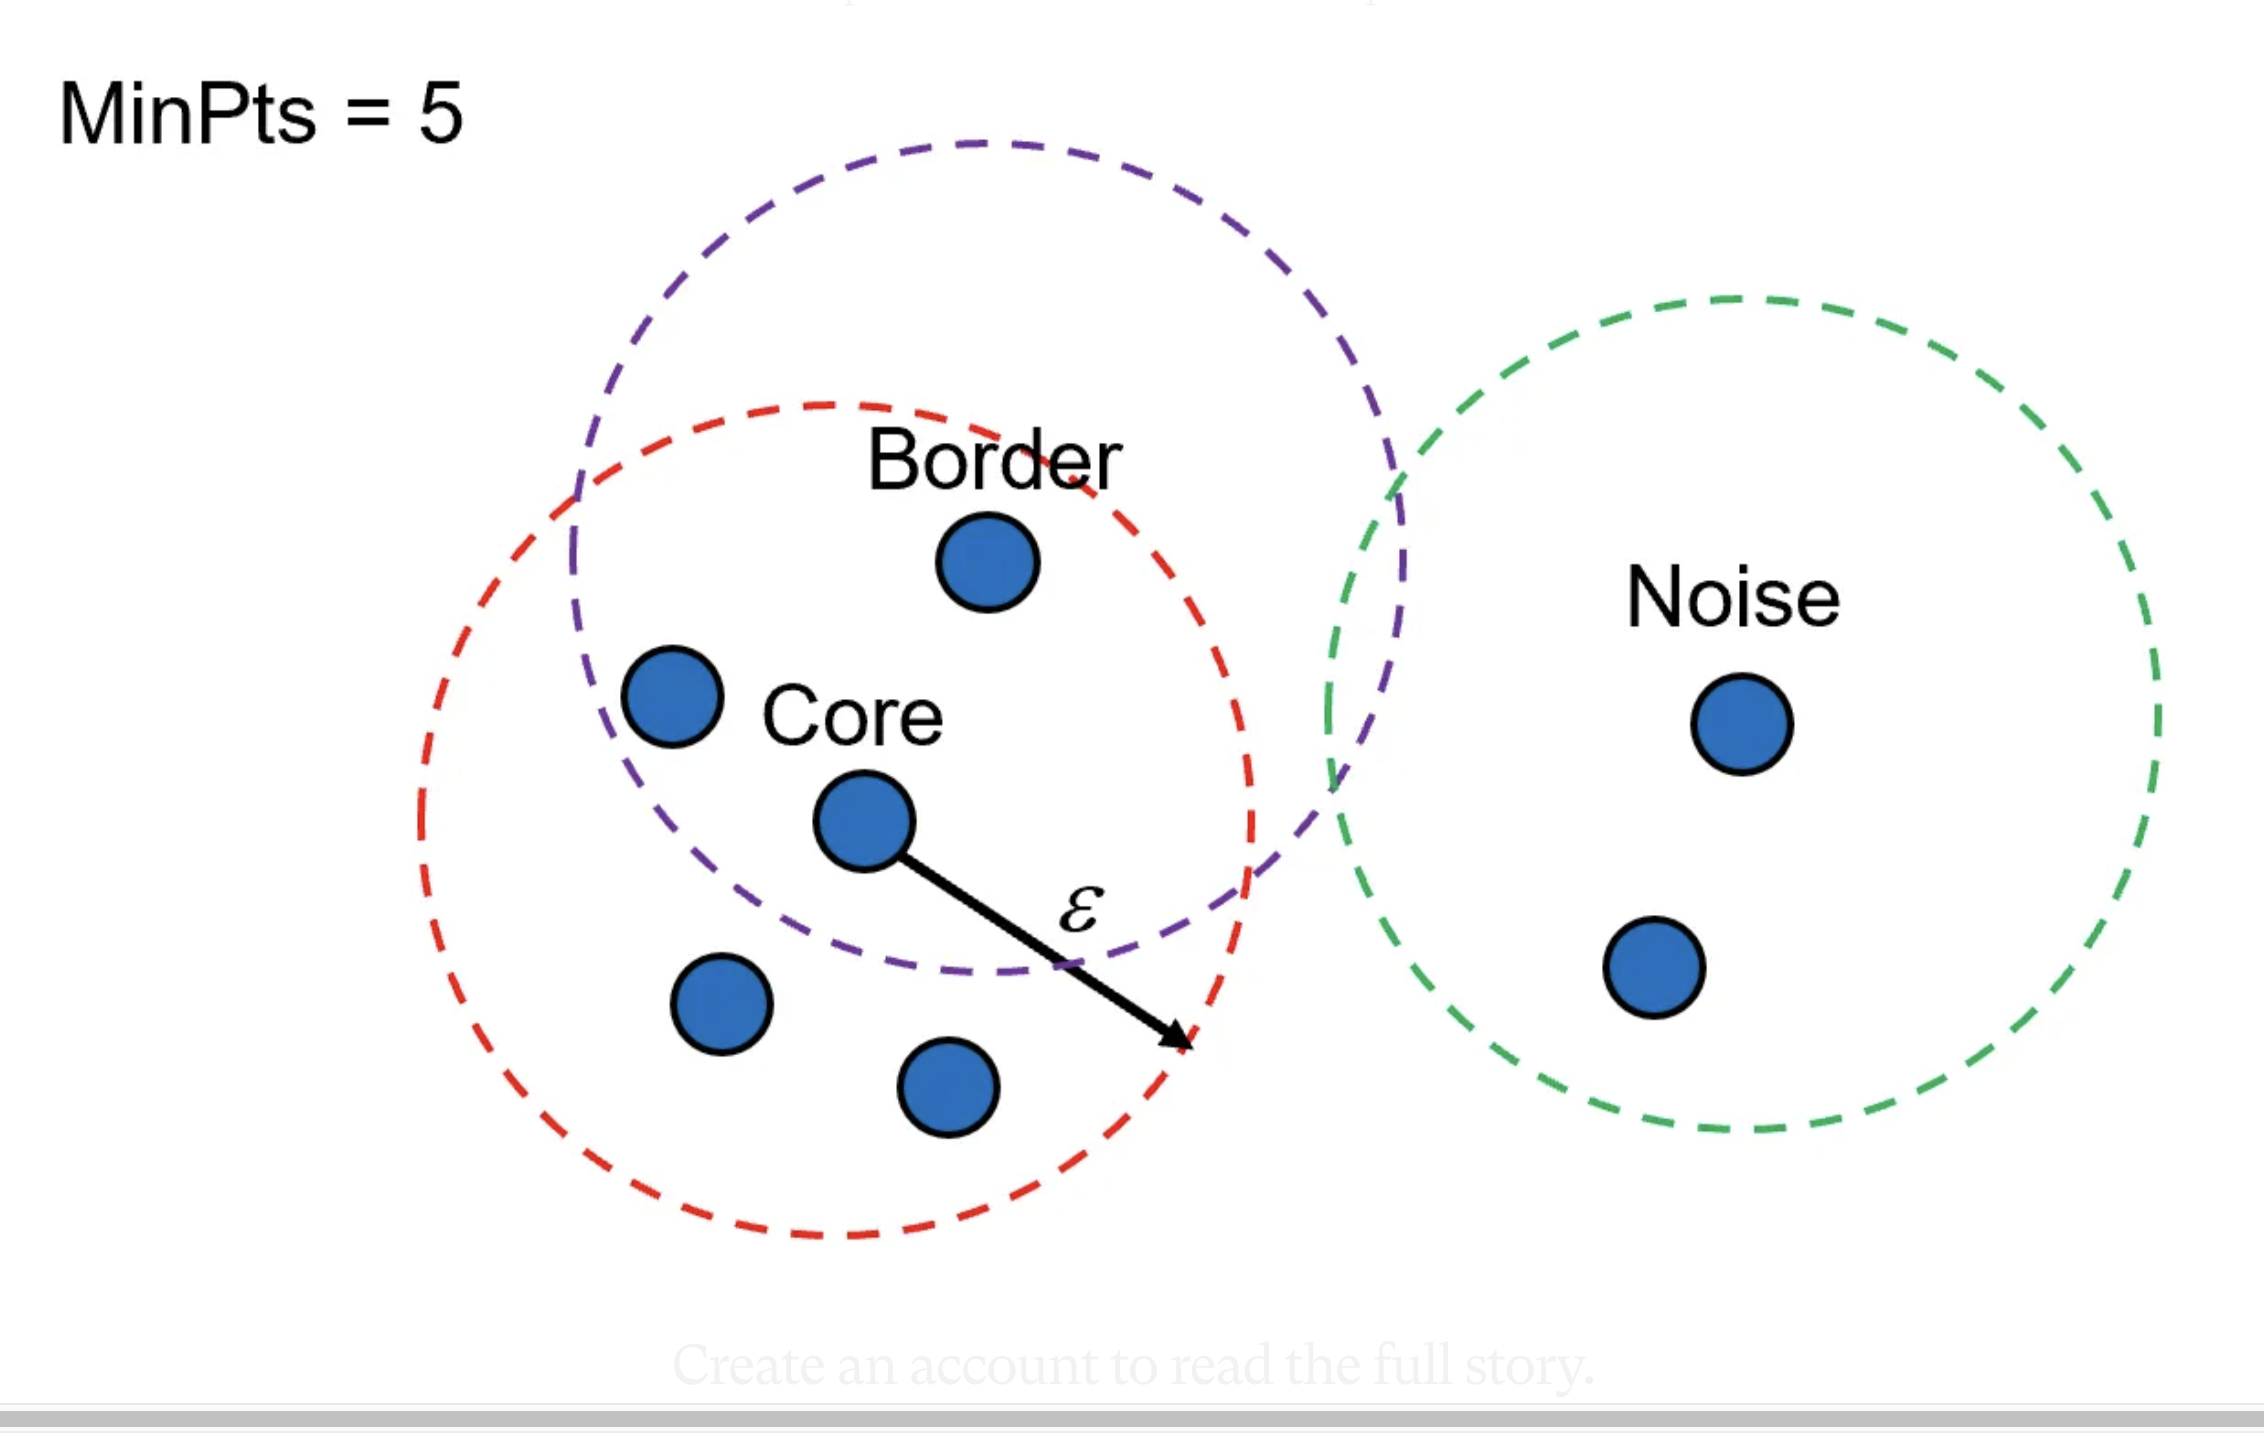
\includegraphics[width=0.55\textwidth]{methods/Screenshot 2026-06-18 at 19.35.24.png} 
    \caption{DBSCAN with MinPts=5}
    \label{fig:autoencoder_architecture}
\end{figure}
Let
\[
X = \{x_1,\ldots,x_n\} \subset \mathbb{R}^p
\]
denote the set of customer-level feature vectors, where each \(x_i\) represents one party. Prior to clustering, all numerical features were standardised to have zero mean and unit variance, since DBSCAN relies on distances between observations.

DBSCAN is controlled by two parameters: the neighbourhood radius \(\varepsilon > 0\) and the minimum number of neighbouring points required to form a dense region, denoted by \(\text{MinPts}\). For a point \(x_i\), its \(\varepsilon\)-neighbourhood is defined as
\[
N_{\varepsilon}(x_i)
=
\left\{
x_j \in X :
d(x_i,x_j) \leq \varepsilon
\right\},
\]
where \(d(\cdot,\cdot)\) is the distance metric. In this project, Euclidean distance was used:
\[
d(x_i,x_j)
=
\left(
\sum_{l=1}^{p}
(x_{il}-x_{jl})^2
\right)^{1/2}.
\]


A point \(x_i\) is defined as a core point if
\[
|N_{\varepsilon}(x_i)| \geq \text{MinPts}.
\]
A point \(x_j\) is directly density-reachable from \(x_i\) if \(x_j \in N_{\varepsilon}(x_i)\) and \(x_i\) is a core point. More generally, \(x_j\) is density-reachable from \(x_i\) if there exists a sequence of points
\[
x_i = z_0, z_1, \ldots, z_m = x_j
\]
such that each \(z_{r+1}\) is directly density-reachable from \(z_r\). A cluster is then defined as a maximal set of density-connected points. Points that are not density-reachable from any core point are labelled as noise.

This distinction is important for money mule detection. The largest dense region is expected to represent common retail behaviour, while noise points and small dense regions may correspond to unusual customer behaviour. Therefore, DBSCAN was used not as a definitive classifier, but as a first-stage segmentation method to reduce the search space and identify accounts requiring further profiling.
\begin{figure} [H]
    \centering
    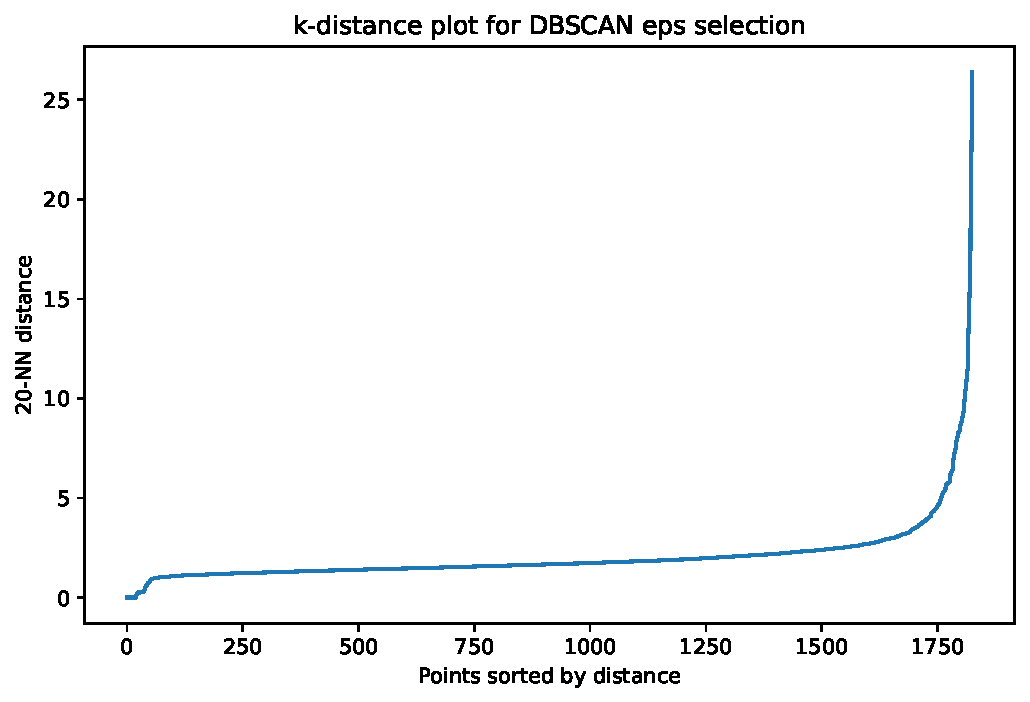
\includegraphics[width=0.55\textwidth]{k_distance_plot.pdf} 
    \caption{k Distance Plot} 
    \label{fig:autoencoder_architecture}
\end{figure}
To guide the choice of \(\varepsilon\), the sorted \(k\)-distance graph heuristic was used, 
as suggested by \cite{ester1996density}. Let $d_k(x_i)$ denote the distance from observation $x_i$ to its $k$-th nearest neighbour, where $k=\text{MinPts}$. Since $\text{MinPts}=20$ in the final implementation, $d_{20}(x_i)$ was computed for every observation. The resulting distances were sorted in ascending order,

\[
d_{(1)} \le d_{(2)} \le \cdots \le d_{(n)},
\]
and plotted against their rank $i$. The horizontal axis therefore represents the ordered index of the observations after sorting, while the vertical axis represents the corresponding $20$-nearest-neighbour distance.

The quantity $d_k(x_i)$ provides a local measure of density around $x_i$. Small values of $d_k(x_i)$ indicate that at least $k$ neighbouring observations lie within a relatively small radius, corresponding to a dense region of the feature space. Conversely, large values indicate that a substantially larger radius is required to encompass $k$ neighbours, suggesting a lower local density.

Equivalently, the DBSCAN core-point condition

\[
|N_{\varepsilon}(x_i)| \ge \text{MinPts}
\]

implies that the distance from $x_i$ to its $k$-th nearest neighbour must satisfy

\[
d_k(x_i) \le \varepsilon.
\]

Consequently, the sorted $k$-distance curve provides information about the distribution of local densities in the dataset. The relatively flat section of the curve corresponds to observations located in dense regions, whereas the rapidly increasing section corresponds to observations in progressively sparser regions. The transition between these two regimes appears as an elbow in the curve.

The parameter $\varepsilon$ was selected near this elbow point. Choosing a substantially smaller value would classify many observations from dense regions as noise, whereas choosing a substantially larger value would merge sparse regions with the main cluster and reduce the ability of DBSCAN to identify anomalous observations. Therefore, the elbow point can be interpreted as an empirical estimate of the density threshold separating the dominant high-density population from lower-density observations. For the present dataset, the elbow occurred at approximately $\varepsilon \approx 4.5/ 5$, which was adopted in the final model.

Sensitivity checks were subsequently performed by comparing the number of clusters and the proportion of noise observations under nearby values of $\varepsilon$.

In the final DBSCAN implementation, \(\text{MinPts}=20\) was used. The selected value of \(\varepsilon\) produced one large cluster representing the majority of retail customers and a smaller set of noise observations. The noise observations were subsequently ranked using mule-behaviour features such as near pass-through ratios, one-in-many-out ratios, and forwarding intensity features.

\section{Autoencoder}

Let
\[
X=\{x_i\}_{i=1}^{n}, \qquad x_i\in\mathbb{R}^{d},
\]
denote the set of account-level feature vectors after preprocessing and
standardisation, where \(d=17\) is the number of input features. Equivalently,
the data matrix may be written as \(X\in\mathbb{R}^{n\times d}\), where each row
corresponds to one account.
\begin{figure}[htbp]
    \centering
    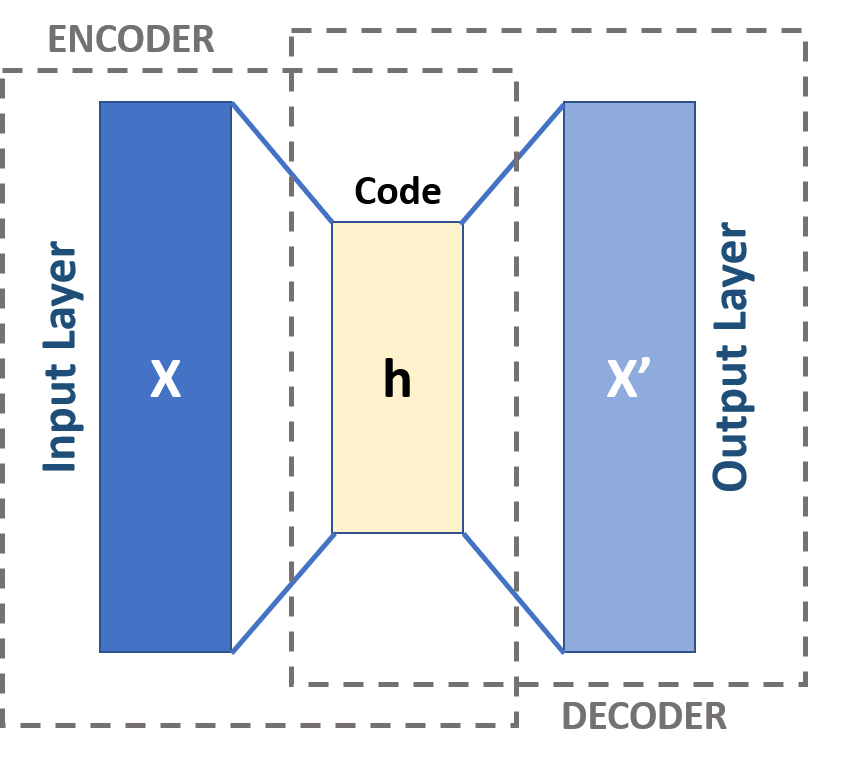
\includegraphics[width=0.55\textwidth]{methods/Autoencoder_schema.png}
    \caption{Schematic representation of an autoencoder architecture.}
    \label{fig:autoencoder_architecture}
\end{figure}
An autoencoder was used as an unsupervised reconstruction model. The objective
of the model is to learn a lower-dimensional representation of each input vector
and then reconstruct the original feature vector from this representation. Let
\[
E_{\phi}:\mathbb{R}^{d}\rightarrow\mathbb{R}^{q}
\]
denote the encoder, where \(\phi\) represents the encoder parameters and
\(q<d\) is the dimension of the latent space. For each observation \(x_i\), the
encoder produces a latent representation
\[
z_i=E_{\phi}(x_i), \qquad z_i\in\mathbb{R}^{q}.
\]
Let
\[
D_{\theta}:\mathbb{R}^{q}\rightarrow\mathbb{R}^{d}
\]
denote the decoder, where \(\theta\) represents the decoder parameters. The
decoder maps the latent representation back to the original feature space:
\[
\hat{x}_i=D_{\theta}(z_i).
\]
Therefore, the full autoencoder mapping is given by
\[
\hat{x}_i=D_{\theta}(E_{\phi}(x_i)).
\]

In this study, the autoencoder was implemented as a fully connected multilayer
perceptron with architecture
\[
17 \rightarrow 8 \rightarrow 4 \rightarrow 8 \rightarrow 17.
\]
The middle layer of dimension \(q=4\) acts as the bottleneck representation. The
hidden layers use the ReLU activation function
\[
\sigma(u)=\max(0,u),
\]
while the output layer is linear, since the task is to reconstruct continuous
standardised features.

More explicitly, the encoder is given by
\[
a_i^{(1)}
=
\sigma\left(W_E^{(1)}x_i+b_E^{(1)}\right),
\]
\[
z_i
=
E_{\phi}(x_i)
=
\sigma\left(W_E^{(2)}a_i^{(1)}+b_E^{(2)}\right),
\]
where
\[
\phi
=
\left\{
W_E^{(1)},b_E^{(1)},W_E^{(2)},b_E^{(2)}
\right\}
\]
denotes the collection of encoder parameters. The decoder is given by
\[
a_i^{(3)}
=
\sigma\left(W_D^{(1)}z_i+b_D^{(1)}\right),
\]
\[
\hat{x}_i
=
D_{\theta}(z_i)
=
W_D^{(2)}a_i^{(3)}+b_D^{(2)},
\]
where
\[
\theta
=
\left\{
W_D^{(1)},b_D^{(1)},W_D^{(2)},b_D^{(2)}
\right\}
\]
denotes the collection of decoder parameters.

The autoencoder is trained by minimising the discrepancy between each input
vector and its reconstruction. In general, the autoencoder objective can be
written as
\[
L(\theta,\phi)
:=
\mathbb{E}_{x\sim\mu_{\mathrm{ref}}}
\left[
d\left(x,D_{\theta}(E_{\phi}(x))\right)
\right],
\]
where \(\mu_{\mathrm{ref}}\) denotes the reference distribution of the training
data and \(d(\cdot,\cdot)\) is a reconstruction distance.

In this implementation, the squared Euclidean distance was used:
\[
d(x,\hat{x})
=
\|x-\hat{x}\|_2^2.
\]
Hence, for the finite training sample \(X=\{x_i\}_{i=1}^{n}\), the empirical
reconstruction loss becomes
\[
\widehat{L}(\theta,\phi)
=
\frac{1}{n}
\sum_{i=1}^{n}
\left\|
x_i-D_{\theta}(E_{\phi}(x_i))
\right\|_2^2.
\]
Equivalently,
\[
\widehat{L}(\theta,\phi)
=
\frac{1}{n}
\sum_{i=1}^{n}
\sum_{j=1}^{d}
\left(x_{ij}-\hat{x}_{ij}\right)^2,
\]
where
\[
\hat{x}_i=D_{\theta}(E_{\phi}(x_i)).
\]
The model was trained using the Adam optimiser with backpropagation. Let
\[
\Theta=(\theta,\phi)
\]
denote the collection of all trainable parameters in the encoder and decoder.
At iteration \(t\), Adam computes a stochastic gradient of the empirical
reconstruction loss over a minibatch \(B_t\):
\[
g_t
=
\nabla_{\Theta}
\left[
\frac{1}{|B_t|}
\sum_{x_i\in B_t}
\left\|
x_i-D_{\theta}(E_{\phi}(x_i))
\right\|_2^2
\right].
\]
Adam maintains exponentially weighted estimates of the first and second moments
of the gradient:
\[
m_t
=
\beta_1 m_{t-1} + (1-\beta_1)g_t,
\]
\[
v_t
=
\beta_2 v_{t-1} + (1-\beta_2)(g_t\odot g_t),
\]
where \(\odot\) denotes element-wise multiplication. The bias-corrected moment
estimates are
\[
\hat{m}_t
=
\frac{m_t}{1-\beta_1^t},
\qquad
\hat{v}_t
=
\frac{v_t}{1-\beta_2^t}.
\]
The parameters are then updated according to
\[
\Theta_t
=
\Theta_{t-1}
-
\eta
\frac{\hat{m}_t}{\sqrt{\hat{v}_t}+\epsilon},
\]
where \(\eta\) is the learning rate and \(\epsilon\) is a small constant used for
numerical stability. In this implementation, the Adam optimiser was used with
learning rate \(\eta=10^{-3}\), \(\beta_1=0.9\), \(\beta_2=0.999\), and
\(\epsilon=10^{-8}\).
```
After training, each account is assigned a reconstruction error score:
\[
s_i
=
\left\|x_i-\hat{x}_i\right\|_2^2
=
\sum_{j=1}^{d}
\left(x_{ij}-\hat{x}_{ij}\right)^2.
\]
Accounts with larger reconstruction errors are interpreted as less well
represented by the patterns learned by the autoencoder. In the context of
anomaly detection, a high reconstruction error suggests that the account's
behaviour differs from the dominant patterns in the training data, and such
accounts are therefore treated as more suspicious candidates for further
investigation.

The underlying assumption is that the majority of accounts in the training data
represent normal behaviour. The autoencoder learns to reconstruct these common
behavioural patterns well, while unusual accounts, such as potential money mule
accounts, are expected to produce larger reconstruction errors.
\section{Supervised Learning}
After the unsupervised experiments, a small set of confirmed mule accounts became available from Novobanco. This allowed an additional supervised modelling experiment to be conducted. The confirmed mule parties were appended to the previously constructed retail party sample, and a binary indicator was created, where confirmed mule parties were assigned label 1 and all remaining sampled retail parties were treated as unlabelled controls with label 0.
Two supervised models were fitted: a class-weighted logistic regression model and a class-weighted XGBoost classifier. Class weighting was used because confirmed mule accounts represented only a small minority of the modelling dataset. This increases the penalty for misclassifying confirmed mule accounts and reduces the tendency of the model to predict the majority unlabelled class for all observations.
\subsection{Logistic Regression}
Logistic regression was used as a supervised linear baseline for binary mule classification. 
It models the conditional probability of the positive class through a logistic transformation 
of a linear predictor, making the log-odds a linear function of the input features 
\citep{cox1958regression}.
Let
\[
x_i \in \mathbb{R}^{p},
\qquad
y_i \in \{0,1\},
\qquad
i=1,\ldots,N,
\]

denote the feature vector and binary label for party \(i\), where \(p\) is the number
of selected behavioural features.

Logistic regression assumes that the log-odds of the positive class is a linear
function of the input variables:

\[
\log
\left(
\frac{\Pr(y_i=1 \mid x_i)}
{\Pr(y_i=0 \mid x_i)}
\right)
=
\beta_0 + x_i^{T}\beta,
\]

where \(\beta_0\) is the intercept and
\(\beta \in \mathbb{R}^{p}\) is the coefficient vector.

Rearranging the above expression yields

\[
p_i
=
\Pr(y_i=1 \mid x_i)
=
\frac{1}
{1+\exp\left[-(\beta_0+x_i^{T}\beta)\right]}.
\]

Under this formulation, the response variable is assumed to follow a Bernoulli
distribution,

\[
y_i \sim \mathrm{Bernoulli}(p_i).
\]

Assuming independent observations, the likelihood function is

\[
L(\beta)
=
\prod_{i=1}^{N}
p_i^{y_i}
(1-p_i)^{1-y_i}.
\]

Taking logarithms gives the log-likelihood

\[
\ell(\beta)
=
\sum_{i=1}^{N}
\left[
y_i \log(p_i)
+
(1-y_i)\log(1-p_i)
\right].
\]

The model parameters were estimated by minimising the negative log-likelihood.
Since confirmed mule accounts represented only a small minority of the modelling
dataset, a class-weighted version of the loss function was used\citep{he2009learning}:

\[
L(\beta)
=
-\sum_{i=1}^{N}
w_{y_i}
\left[
y_i \log(p_i) + (1-y_i)\log(1-p_i)
\right]
+
\lambda \|\beta\|_2^2,
\]

where \(\lambda \|\beta\|_2^2\) denotes the \(L_2\) regularisation penalty, which shrinks large coefficients and helps stabilise the model when behavioural features are correlated.  \(w_{y_i}\) denotes the class weight assigned to observation \(i\).
For the scikit-learn implementation \cite{sklearn_logistic} with \texttt{class\_weight="balanced"}, the class weight for class \(c\) is defined as
\[
w_c = \frac{N}{K N_c} ,
\]
where \(N\) is the number of training observations, \(K\) is the number of classes, and \(N_c\) is the number of observations belonging to class \(c\) in the training set. In this experiment, the training set contained 1506 unlabeled observations and 72 confirmed mule observations. Therefore, the corresponding class weights were
\[
w_0 = \frac{1578}{2 \times 1506} \approx 0.524,
\qquad
w_1 = \frac{1578}{2 \times 72} \approx 10.958.
\]

Thus, errors on confirmed mule observations received substantially larger weight than errors on unlabeled observations. This was intended to reduce the tendency of the model to favour the majority unlabeled class and to improve sensitivity to the minority confirmed mule class.


The model was implemented using the \texttt{LogisticRegression} estimator from
the \texttt{scikit-learn} package with \texttt{class\_weight="balanced"}.
The optimisation of the coefficient vector was performed automatically by the
underlying numerical optimisation algorithm.
\subsection{XGBoost}
As a second supervised baseline, an XGBoost classifier was used. XGBoost, introduced by \cite{Chen_2016}, is a scalable gradient tree boosting method that constructs an additive ensemble of decision trees. While logistic
regression models the log-odds as a linear function of the input features, XGBoost
constructs a non-linear additive model of decision trees. This makes it suitable for
capturing interaction effects between behavioural features, such as high draining
activity combined with one-in-many-out transfer patterns.

Let \(x_i \in \mathbb{R}^{p}\) denote the feature vector for party \(i\), and let
\(y_i \in \{0,1\}\) denote the binary label. XGBoost models the prediction as an
additive ensemble of regression trees,

\[
\hat{z}_i
=
\sum_{k=1}^{K} f_k(x_i),
\qquad
f_k \in \mathcal{F},
\]

where \(\mathcal{F}\) denotes the space of regression trees and \(\hat{z}_i\) is the
raw prediction score before applying the logistic transformation. For binary
classification, the predicted probability of the positive class is obtained by

\[
\hat{p}_i
=
\sigma(\hat{z}_i)
=
\frac{1}{1+\exp(-\hat{z}_i)}.
\]

The objective function consists of a training loss and a regularisation penalty on
the complexity of the trees:

\[
\mathcal{L}
=
\sum_{i=1}^{N}
l(y_i,\hat{p}_i)
+
\sum_{k=1}^{K}
\Omega(f_k),
\]

where \(l(y_i,\hat{p}_i)\) is the binary logistic loss,

\[
l(y_i,\hat{p}_i)
=
-
\left[
y_i\log(\hat{p}_i)
+
(1-y_i)\log(1-\hat{p}_i)
\right].
\]

The regularisation term penalises overly complex trees and is commonly written as

\[
\Omega(f)
=
\gamma T
+
\frac{1}{2}\lambda
\sum_{j=1}^{T}
w_j^2,
\]

where \(T\) is the number of leaves in the tree, \(w_j\) is the score assigned to
leaf \(j\), and \(\gamma\) and \(\lambda\) are regularisation parameters.

XGBoost fits trees sequentially. Suppose that after \(t-1\) boosting iterations the
current raw prediction for observation \(i\) is \(\hat{z}_i^{(t-1)}\). At iteration
\(t\), a new tree \(f_t\) is added, giving

\[
\hat{z}_i^{(t)}
=
\hat{z}_i^{(t-1)}
+
f_t(x_i).
\]

The objective at iteration \(t\) is therefore

\[
\mathcal{L}^{(t)}
=
\sum_{i=1}^{N}
l\left(y_i,\sigma\left(\hat{z}_i^{(t-1)}+f_t(x_i)\right)\right)
+
\Omega(f_t).
\]

Rather than optimising this objective directly, XGBoost uses a second-order Taylor
approximation of the loss around the current predictions:

\[
\mathcal{L}^{(t)}
\approx
\sum_{i=1}^{N}
\left[
g_i f_t(x_i)
+
\frac{1}{2}h_i f_t(x_i)^2
\right]
+
\Omega(f_t),
\]

where

\[
g_i
=
\frac{\partial l(y_i,\hat{p}_i)}
{\partial \hat{z}_i},
\qquad
h_i
=
\frac{\partial^2 l(y_i,\hat{p}_i)}
{\partial \hat{z}_i^2}.
\]

For logistic loss, these terms are

\[
g_i = \hat{p}_i - y_i,
\qquad
h_i = \hat{p}_i(1-\hat{p}_i).
\]

Each tree partitions the observations into leaves. Let \(I_j\) denote the set of
observations assigned to leaf \(j\). The sum of first-order and second-order
gradient statistics in leaf \(j\) are

\[
G_j = \sum_{i \in I_j} g_i,
\qquad
H_j = \sum_{i \in I_j} h_i.
\]

For a fixed tree structure, the optimal leaf weight is

\[
w_j^{*}
=
-
\frac{G_j}{H_j+\lambda}.
\]

Substituting this back into the objective gives the approximate optimal value of a
tree:

\[
\tilde{\mathcal{L}}^{(t)}
=
-
\frac{1}{2}
\sum_{j=1}^{T}
\frac{G_j^2}{H_j+\lambda}
+
\gamma T.
\]

This expression shows how XGBoost chooses splits. For a candidate split dividing a
node into left and right child nodes, the split gain is

\[
\mathrm{Gain}
=
\frac{1}{2}
\left[
\frac{G_L^2}{H_L+\lambda}
+
\frac{G_R^2}{H_R+\lambda}
-
\frac{(G_L+G_R)^2}{H_L+H_R+\lambda}
\right]
-
\gamma.
\]

A split is selected when it provides a positive improvement in the regularised
objective. This mechanism allows XGBoost to build trees greedily while controlling
overfitting through the regularisation parameters.

Since confirmed mule accounts formed only a small minority of the modelling dataset, class
imbalance was handled using the parameter \texttt{scale\_pos\_weight}. This parameter increases the
contribution of positive observations in the training objective. In the implementation \cite{xgboost_parameters} , it was set
as
\[
\texttt{scale\_pos\_weight} = \frac{N_0}{N_1},
\]
where \(N_0\) is the number of unlabeled observations and \(N_1\) is the number of confirmed mule
observations in the training set. In this experiment, the training set contained 1506 unlabeled
observations and 72 confirmed mule observations. Therefore,
\[
\texttt{scale\_pos\_weight}
=
\frac{1506}{72}
\approx 20.92.
\]
This gives greater weight to confirmed mule observations during training and reduces the
tendency of the model to favour the majority unlabeled class.
The model was implemented using the \texttt{XGBClassifier} estimator. As with the
logistic regression model, the output scores were interpreted as relative mule-risk
scores rather than calibrated probabilities, since the confirmed mule accounts were
appended to a random retail sample.

To interpret the XGBoost model, SHAP values were computed as a post-hoc explanation method. SHAP is based on Shapley values from cooperative game theory and decomposes each model prediction into additive feature contributions \citep{lundberg2017unified}. For an observation \(i\), the model output can be written as
\[
f(x_i) = \mathbb{E}[f(X)] + \sum_{j=1}^{p} \phi_{ij},
\]
where \(\mathbb{E}[f(X)]\) is the baseline model output and \(\phi_{ij}\) is the SHAP value of feature \(j\) for observation \(i\). A positive SHAP value indicates that the feature pushes the prediction towards the confirmed mule class, while a negative SHAP value pushes the prediction towards the unlabeled comparison class. Global feature importance was measured using the mean absolute SHAP value,
\[
I_j = \frac{1}{N}\sum_{i=1}^{N} |\phi_{ij}|.
\]
The SHAP summary plot was used to visualise both the magnitude and direction of feature effects for the XGBoost classifier.
\chapter{Results}
\section{DBSCAN Results}

Using the selected value of \(\varepsilon=4.5\) and
\(\texttt{min\_samples}=20\),
DBSCAN identified one large cluster and a set of noise observations.

\begin{table}[H]
\centering
\begin{tabular}{lcc}
\hline
Cluster & Accounts & Proportion \\
\hline
Cluster 0 & 1777 & 97.3\% \\
Noise (-1) & 49 & 2.7\% \\
\hline
\end{tabular}
\caption{DBSCAN cluster sizes.}
\end{table}
\begin{table}[H]
\centering
\small
\begin{tabular}{lcc}
\hline
Feature & Cluster 0 & Noise (-1) \\
\hline
Transactions per active day & 2.858 & 12.551 \\
Log outgoing amount per span day & 3.927 & 5.812 \\
Outgoing transaction ratio & 0.747 & 0.717 \\
Outgoing amount ratio & 0.507 & 0.594 \\
Off-hours ratio & 0.619 & 0.592 \\
Weekend ratio & 0.196 & 0.171 \\
Mean-to-median amount ratio & 0.622 & 0.625 \\
P90-to-median amount ratio & 15.320 & 484.870 \\
Max-to-median amount ratio & 363.317 & 5474.357 \\
Near pass-through ratio (1h) & 0.018 & 0.144 \\
Near pass-through ratio (24h) & 0.061 & 0.253 \\
One-in-many-out ratio (1h) & 0.006 & 0.029 \\
One-in-many-out ratio (24h) & 0.267 & 0.446 \\
Drain ratio (1h) & 0.007 & 0.183 \\
Drain ratio (24h) & 0.157 & 0.502 \\
\hline
\end{tabular}
\caption{Mean feature values for Cluster 0 and the DBSCAN noise group.}
\label{tab:dbscan_profile}
\end{table}
The majority of retail parties were assigned to a single large cluster,
which may be interpreted as the dominant pattern of normal account
behaviour. A small number of observations were classified as noise and
were therefore considered anomalous under the density-based clustering
framework.

Table \ref{tab:dbscan_profile} shows the mean feature values for the main DBSCAN cluster and the noise observations.

The noise group exhibits substantially higher transaction intensity, with an average of 12.55 transactions per active day compared with 2.86 for Cluster 0. The noise observations also display stronger pass-through behaviour, higher drain ratios, and larger one-in-many-out ratios across both the 1-hour and 24-hour windows.

In addition, the noise accounts show considerably more extreme transaction size distributions. The median-normalised upper-tail statistics (\texttt{p90\_median\_ratio} and \texttt{max\_median\_ratio}) are substantially larger than those observed in Cluster 0, indicating the presence of occasional unusually large transactions.

Overall, the noise observations exhibit behavioural characteristics that are more consistent with potential money mule activity than the accounts contained within the large normal cluster.

The largest difference was observed for transaction intensity.
Noise observations exhibited substantially higher values of
\texttt{txn\_per\_active\_day}
(4.70 compared with 0.18 in the main cluster),
indicating a much higher concentration of transactional activity.

Noise observations also displayed stronger one-in-many-out behaviour.
The average value of
\texttt{one\_in\_many\_out\_24h\_ratio}
was 0.45 for the noise accounts,
compared with 0.27 for accounts in the main cluster.

Similarly, pass-through behaviour was more pronounced within the noise
group.
The average
\texttt{near\_pass\_through\_24h\_ratio}
was approximately three times larger than that observed in the main
cluster.

Finally, noise observations exhibited substantially larger values of
\texttt{max\_out\_txn\_after\_in\_1h},
suggesting that incoming funds were frequently followed by multiple
outgoing transfers within a short time window.

These results indicate that the accounts identified as noise tend to
exhibit characteristics commonly associated with money mule behaviour,
including rapid redistribution of funds and elevated transaction
activity.
To identify the features that most strongly characterised the DBSCAN noise group,
cluster-level feature means were compared with the corresponding global feature
distributions. For each feature \(j\), a standardised deviation score was computed as

\begin{equation*}
z_{c,j}
=
\frac{\mu_{c,j}-\mu_j}{\sigma_j},
\end{equation*}

where \(\mu_{c,j}\) denotes the mean of feature \(j\) within cluster \(c\),
\(\mu_j\) denotes the mean of feature \(j\) over the full dataset, and
\(\sigma_j\) denotes the corresponding global standard deviation.

For the noise group \(c=-1\), features were ranked by the absolute value
\(|z_{-1,j}|\). Larger values indicate that the average value of that feature
within the noise group deviates more strongly from the overall population mean.

\begin{table}[H]
\centering
\begin{tabular}{lc}
\hline
Feature & Noise z-score \\
\hline
drain\_ratio\_1h & 2.699 \\
txn\_per\_active\_day & 2.413 \\
near\_pass\_through\_24h\_ratio & 2.067 \\
max\_median\_ratio & 2.047 \\
near\_pass\_through\_1h\_ratio & 1.895 \\
drain\_ratio\_24h & 1.827 \\
one\_in\_many\_out\_24h\_ratio & 1.076 \\
log\_outgoing\_amount\_per\_span\_day & 0.941 \\
p90\_median\_ratio & 0.828 \\
one\_in\_many\_out\_1h\_ratio & 0.617 \\
\hline
\end{tabular}
\caption{Top feature drivers for the DBSCAN noise group.}
\label{tab:dbscan_top_drivers}
\end{table}

\section{Autoencoder Results}
For both autoencoder experiments, model behaviour was assessed using two quantities.
First, the training loss measures the reconstruction error on the training set. A decreasing
training loss indicates that the network is learning a mapping from the input features to
their reconstructions.

Second, the validation score reported by \texttt{MLPRegressor} corresponds to the
coefficient of determination, \(R^2\), evaluated on a held-out validation set. This measures
the reconstruction quality on unseen observations, with values closer to one indicating
better reconstruction performance. Therefore, while the training loss describes how well
the model fits the training data, the validation score provides information about whether
the learned reconstruction function generalises beyond the training sample.

In the context of anomaly detection, this distinction is important. A useful reconstruction
model should reconstruct normal-like observations well, while assigning larger
reconstruction errors to observations that deviate from the learned normal pattern.

\subsection{Autoencoder Trained on the Full Dataset}

The first experiment trained the autoencoder using all 1,826 accounts in the dataset. 
The objective was to evaluate whether the model could learn a compact representation of 
the overall population without any prior filtering of anomalous observations.

The autoencoder architecture consisted of an encoder-decoder structure with hidden layer sizes
$(8,4,8)$ and ReLU activation functions. Training was performed using the Adam optimiser
with early stopping based on validation performance.
\begin{figure}[H]
\centering
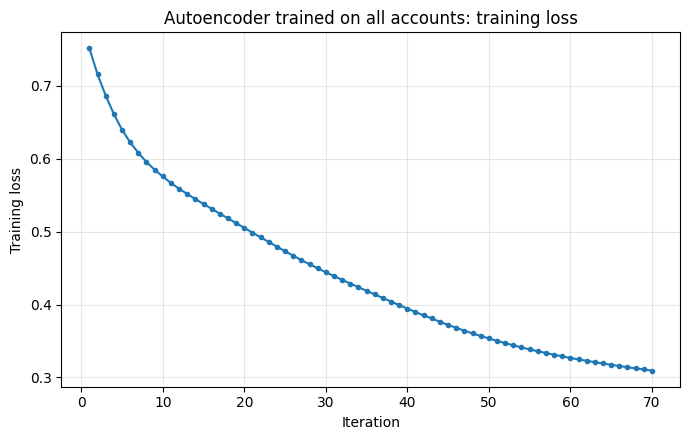
\includegraphics[width=0.75\textwidth]{results/output.png}
\caption{Training loss for the autoencoder trained on the full dataset.}
\label{fig:ae_all_loss}
\end{figure}
Figure~\ref{fig:ae_all_loss} shows the evolution of the reconstruction loss during training.
The loss decreases monotonically from approximately 0.75 to 0.31, indicating that the model
successfully learned to reconstruct the training observations.

However, a decreasing training loss alone does not imply that the learned representation
generalises well to unseen observations. Validation performance must also be examined.
\begin{figure}[H]
\centering
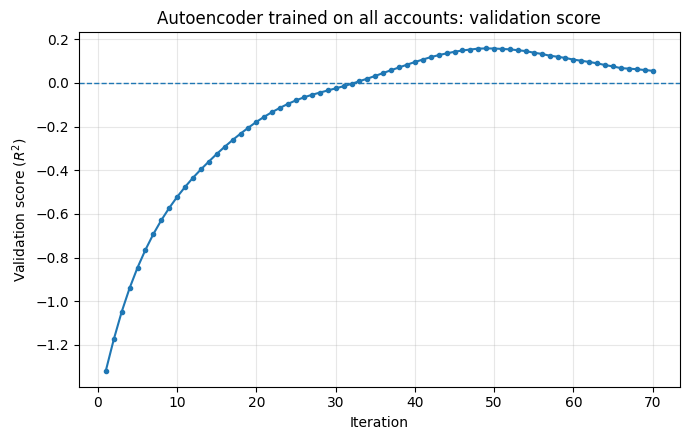
\includegraphics[width=0.75\textwidth]{results/output (1).png}
\caption{Validation score for the autoencoder trained on the full dataset.}
\label{fig:ae_all_val}
\end{figure}
Figure~\ref{fig:ae_all_val} presents the validation score reported by the
\texttt{MLPRegressor} implementation. The score corresponds to the coefficient of
determination ($R^2$) between the reconstructed and original feature vectors.

Although the validation score improves steadily throughout training, the best value obtained
is approximately 0.16. This indicates that only a relatively small proportion of the variation
in the validation observations is explained by the reconstructed outputs.

Consequently, the autoencoder exhibits limited reconstruction capability when trained on the
entire dataset. One possible explanation is that the training set contains both normal and
anomalous accounts, making it difficult for a single latent representation to accurately model
the dominant behaviour patterns.

To address this issue, a second experiment was conducted using only accounts belonging to
the large DBSCAN cluster identified before. Since this cluster contains the vast
majority of observations and is assumed to represent normal account behaviour, training the
autoencoder exclusively on this subset may allow the model to learn a cleaner representation
of normal activity patterns.

\subsection{Autoencoder Trained on Cluster 0}
The autoencoder trained only on DBSCAN Cluster 0 showed substantially improved reconstruction performance compared with the model trained on the full sample. The training loss decreased steadily from approximately \(0.737\) to \(0.149\), indicating that the network was able to reduce reconstruction error on the training data. At the same time, the validation score increased from a negative value to approximately \(R^2=0.704\), suggesting that the model also generalised well to unseen observations from Cluster 0.
\begin{figure}[H]
\centering
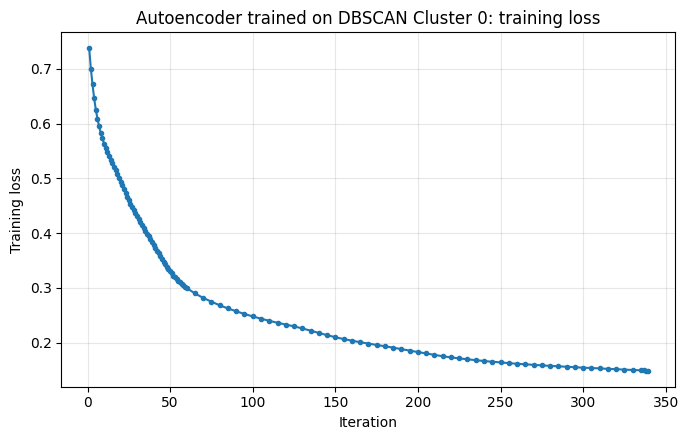
\includegraphics[width=0.75\textwidth]{results/output (2).png}
\caption{Training loss for the autoencoder trained on DBSCAN cluster 0.}
\label{fig:ae_all_val}
\end{figure}

\begin{figure}[H]
\centering
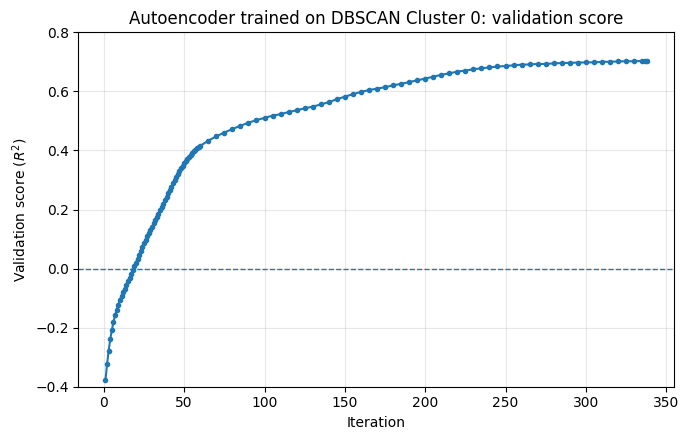
\includegraphics[width=0.75\textwidth]{results/output (4).png}
\caption{Training score for the autoencoder trained on DBSCAN cluster 0.}
\label{fig:ae_all_val}
\end{figure}
This supports the interpretation that Cluster 0 forms a more homogeneous approximation of normal account behaviour. In contrast, training the autoencoder on the full sample forced the model to reconstruct a more heterogeneous population, including noise observations, which led to much weaker validation performance. Therefore, the Cluster 0 autoencoder was used as the main reconstruction model for anomaly scoring.
\subsection{Manual Anomaly Injection Stress Test}

To further compare the anomaly sensitivity of the two autoencoder specifications, a manual anomaly injection experiment was conducted. A random 5\% of observations were selected from the sample and their feature values were modified to represent synthetic abnormal behaviours. This experiment was not intended as a formal evaluation of real money mule detection performance, since the injected observations are artificially constructed. Instead, it was used as a stress test to assess whether each autoencoder assigns high reconstruction errors to observations with clearly abnormal feature patterns.

Three types of synthetic anomalies were introduced. The first type represents mule-like pass-through behaviour. These observations were assigned high values for features such as the outgoing amount ratio, short-window drain ratio, near pass-through ratio, and one-in-many-out ratio. This corresponds to accounts where incoming funds are rapidly transferred out, often in amounts close to the incoming value. The second type represents burst behaviour, where transaction intensity and maximum-to-median amount ratios were increased. This captures accounts that suddenly become unusually active or receive unusually large transactions relative to their typical transaction size. The third type represents abnormal timing behaviour, where off-hours and weekend transaction ratios were increased, corresponding to accounts whose activity is concentrated outside normal working patterns.

After injecting the anomalies, both autoencoders were used to score all observations by reconstruction error. The top 20\% highest-error observations were then selected, and the number of injected anomalies recovered within this top-ranked group was recorded. The results are reported in Table~\ref{tab:ae_injection_test}.

\begin{table}[H]
\centering
\begin{tabular}{lcccc}
\hline
Model & Injected anomalies & Top 20\% size & Detected in top 20\% & Detection rate \\
\hline
AE trained on full sample & 91 & 365 & 28 & 30.8\% \\
AE trained on Cluster 0 & 91 & 365 & 60 & 65.9\% \\
\hline
\end{tabular}
\caption{Manual anomaly injection stress test for the two autoencoder models.}
\label{tab:ae_injection_test}
\end{table}

The autoencoder trained on Cluster 0 recovered 60 out of the 91 injected anomalies within the top 20\% reconstruction-error ranking, compared with 28 out of 91 for the autoencoder trained on the full sample. This indicates that the Cluster 0 autoencoder is substantially more sensitive to the injected abnormal behaviours. This result is consistent with the interpretation that Cluster 0 provides a cleaner approximation of normal account behaviour. Since the full-sample autoencoder is trained on a more heterogeneous population, including potentially noisy or unusual observations, it may learn to reconstruct a wider range of behaviours and therefore assign lower anomaly scores to some abnormal cases. In contrast, the Cluster 0 autoencoder learns a narrower normal reconstruction pattern, causing mule-like, burst, and timing anomalies to produce larger reconstruction errors.



\subsection{Supervised Learning Models}

In addition to the unsupervised anomaly detection methods, supervised baseline models were trained using the available confirmed mule labels. Confirmed mule accounts were treated as positive observations. Since verified non-mule labels were not available, the remaining sampled accounts were used as an unlabeled comparison group and were assigned label 0 for training purposes. Therefore, these models should be interpreted as label-informed baselines rather than fully validated mule-versus-non-mule classifiers.

Class weighting was used to account for the strong imbalance between the confirmed mule accounts and the unlabeled comparison group. The training set contained 72 confirmed mule observations and 1506 unlabeled observations, while the test set contained 20 confirmed mule observations and 320 unlabeled observations.

\subsubsection{Logistic Regression Results}

Logistic regression was used as an interpretable linear supervised baseline. The model estimates the log-odds of an account being a confirmed mule as a linear function of the engineered behavioural features. The classification report for the held-out test set is shown in Table~\ref{tab:logistic_classification_report}.

\begin{table}[H]
\centering
\begin{tabular}{lcccc}
\hline
Class & Precision & Recall & F1-score & Support \\
\hline
Unlabeled comparison group & 0.99 & 0.85 & 0.92 & 320 \\
Confirmed mule & 0.28 & 0.90 & 0.42 & 20 \\
\hline
Accuracy & \multicolumn{3}{c}{0.86} & 340 \\
Macro average & 0.63 & 0.88 & 0.67 & 340 \\
Weighted average & 0.95 & 0.86 & 0.89 & 340 \\
\hline
\end{tabular}
\caption{Classification report for the logistic regression supervised baseline.}
\label{tab:logistic_classification_report}
\end{table}

The logistic regression model achieved high recall for the confirmed mule class, correctly identifying 18 out of 20 confirmed mule accounts. However, its mule-class precision was relatively low at 0.28, meaning that a relatively large number of unlabeled accounts were also classified as mule-like. In the context of this study, these should not be interpreted as definitive false positives, since the unlabeled comparison group may contain hidden mule accounts. Instead, the result suggests that logistic regression is sensitive to mule-like behaviour but produces a broad suspicious-account ranking.
\begin{table}[H]
\centering
\begin{tabular}{lrr}
\hline
Feature & Coefficient & Absolute coefficient \\
\hline
drain\_ratio\_24h & 3.6739 & 3.6739 \\
outgoing\_txn\_ratio & -3.5964 & 3.5964 \\
outgoing\_amount\_ratio & -2.9349 & 2.9349 \\
one\_in\_many\_out\_24h\_ratio & 2.9615 & 2.9615 \\
mean\_median\_gap\_ratio & 1.5067 & 1.5067 \\
offhours\_ratio & 0.6305 & 0.6305 \\
log\_outgoing\_amount\_per\_span\_day & 0.4952 & 0.4952 \\
weekend\_ratio & 0.3982 & 0.3982 \\
max\_out\_method\_div\_after\_in\_1h & -0.1547 & 0.1547 \\
one\_in\_many\_out\_1h\_ratio & -0.1254 & 0.1254 \\
drain\_ratio\_1h & 0.0952 & 0.0952 \\
max\_out\_txn\_after\_in\_1h & 0.0831 & 0.0831 \\
near\_pass\_through\_24h\_ratio & 0.0708 & 0.0708 \\
txn\_per\_active\_day & -0.0396 & 0.0396 \\
near\_pass\_through\_1h\_ratio & 0.0195 & 0.0195 \\
max\_out\_txn\_after\_in\_24h & -0.0070 & 0.0070 \\
max\_median\_ratio & -0.0002 & 0.0002 \\
\hline
\end{tabular}
\caption{Logistic regression coefficients ranked by absolute coefficient magnitude.}
\label{tab:logistic_feature_importance}
\end{table}
The strongest positive coefficient was obtained for drain\_ratio\_24h, followed by one\_in\_many\_out\_24h\_ratio. This suggests that, within the fitted logistic regression model, accounts showing stronger 24-hour draining behaviour and one-in-many-out transfer patterns were assigned higher mule-risk scores. This is consistent with the expected behaviour of mule accounts, where incoming funds are rapidly forwarded to other destinations.

These negative coefficients should be interpreted cautiously. They do not necessarily imply that outgoing activity is protective. Instead, after more specific mule-behaviour variables such as drain\_ratio\_24h and one\_in\_many\_out\_24h\_ratio are included, the generic outgoing ratios may capture a different type of activity, such as normally active retail accounts with frequent outgoing payments but without clear draining behaviour.

In regression models, correlated predictors can make individual coefficient estimates less stable and may even lead to coefficient sign reversals or suppression effects 
\citep{vatcheva2016multicollinearity,ludlow2014suppressor}. Therefore, the coefficient 
ranking is used as a model-specific diagnostic of feature contribution rather than as formal 
evidence of individual feature significance.
\subsubsection{XGBoost Results}

XGBoost was used as a nonlinear supervised benchmark. Unlike logistic regression, it can capture threshold effects and interactions between behavioural features, which may be important in money mule detection because suspicious behaviour often depends on combinations of rapid drainage, pass-through ratios, transaction intensity, and unusual timing patterns. The classification report for the held-out test set is shown in Table~\ref{tab:xgboost_classification_report}.

\begin{table}[H]
\centering
\begin{tabular}{lcccc}
\hline
Class & Precision & Recall & F1-score & Support \\
\hline
Unlabeled comparison group & 0.98 & 0.99 & 0.99 & 320 \\
Confirmed mule & 0.79 & 0.75 & 0.77 & 20 \\
\hline
Accuracy & \multicolumn{3}{c}{0.97} & 340 \\
Macro average & 0.89 & 0.87 & 0.88 & 340 \\
Weighted average & 0.97 & 0.97 & 0.97 & 340 \\
\hline
\end{tabular}
\caption{Classification report for the XGBoost supervised baseline.}
\label{tab:xgboost_classification_report}
\end{table}

The XGBoost model achieved a more balanced performance than logistic regression. It identified 15 out of 20 confirmed mule accounts while producing only 4 positive predictions among the unlabeled comparison group. This resulted in a confirmed-mule precision of 0.79 and recall of 0.75. Therefore, XGBoost provided a stronger supervised predictive ranking, especially in terms of precision.
\begin{table}[H]
\centering
\begin{tabular}{lr}
\hline
Feature & Importance \\
\hline
txn\_per\_active\_day & 0.2192 \\
drain\_ratio\_24h & 0.1212 \\
log\_outgoing\_amount\_per\_span\_day & 0.0794 \\
outgoing\_txn\_ratio & 0.0737 \\
max\_out\_txn\_after\_in\_1h & 0.0481 \\
mean\_median\_gap\_ratio & 0.0457 \\
outgoing\_amount\_ratio & 0.0445 \\
one\_in\_many\_out\_24h\_ratio & 0.0419 \\
max\_median\_ratio & 0.0410 \\
offhours\_ratio & 0.0407 \\
drain\_ratio\_1h & 0.0382 \\
max\_out\_method\_div\_after\_in\_1h & 0.0371 \\
weekend\_ratio & 0.0368 \\
max\_out\_txn\_after\_in\_24h & 0.0336 \\
near\_pass\_through\_24h\_ratio & 0.0302 \\
near\_pass\_through\_1h\_ratio & 0.0292 \\
\hline
\end{tabular}
\caption{XGBoost "Gain" feature importance values.}
\label{tab:xgboost_feature_importance}
\end{table}
\begin{figure}[htbp]
    \centering
    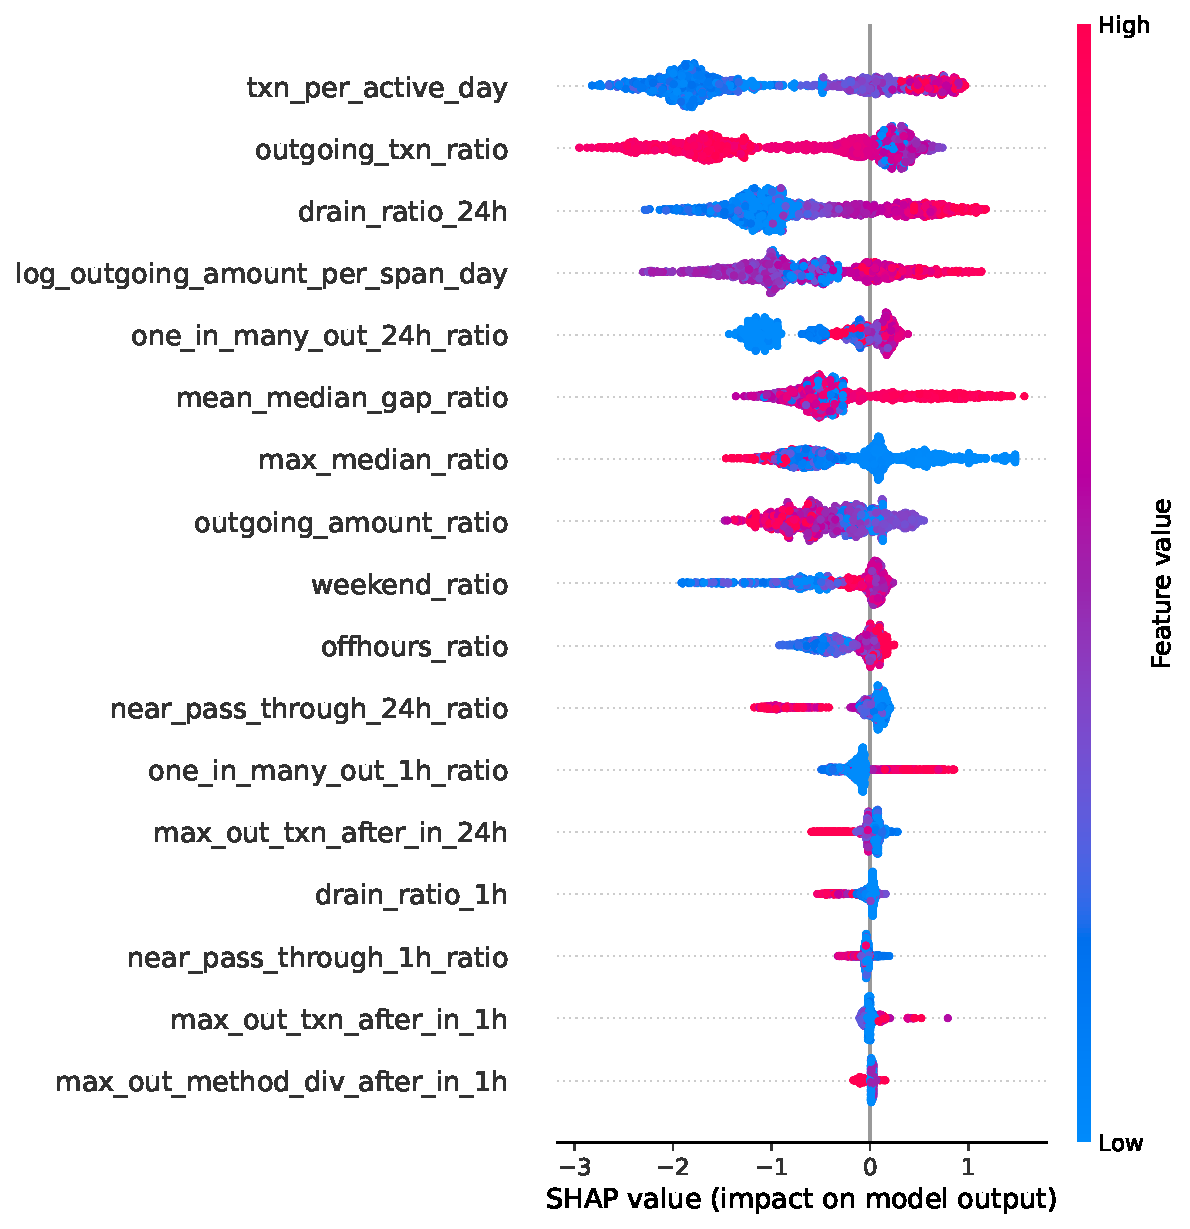
\includegraphics[width=0.55\textwidth]{methods/shap_summary_plot.pdf}
    \caption{SHAP summary plot for the XGBoost classifier.}
\end{figure}
Figure 6.5 presents the SHAP summary plot for the XGBoost classifier. The features are ranked by their mean absolute SHAP values, so variables appearing higher in the plot have a larger average impact on the model output. Each point represents one observation. The horizontal position shows the SHAP value, where positive values push the prediction towards the confirmed mule class and negative values push it towards the unlabeled comparison class. The colour indicates the feature value, with red corresponding to high feature values and blue corresponding to low feature values.

The most influential variable was \texttt{txn\_per\_active\_day}, indicating that transaction frequency per active day had the largest average impact on the XGBoost predictions. Higher values of this feature generally pushed the model output towards the confirmed mule class, suggesting that the model associated higher transaction intensity with greater mule risk. However, this variable is not mule-specific and may also capture generally active retail behaviour.

More mule-specific behavioural features also appeared among the most important variables. High values of \texttt{drain\_ratio\_24h} generally produced positive SHAP values, meaning that stronger 24-hour draining behaviour increased the predicted mule-risk score. Similarly, high values of \texttt{one\_in\_many\_out\_24h\_ratio} tended to push predictions towards the confirmed mule class. These patterns are consistent with the expected behaviour of money mule accounts, where incoming funds are rapidly forwarded onwards, sometimes through multiple outgoing transfers.

By contrast, \texttt{outgoing\_txn\_ratio} showed a negative effect for high feature values, with high values tending to push the prediction away from the confirmed mule class. This should not be interpreted as evidence that outgoing activity is inherently non-suspicious. Rather, after accounting for more targeted mule-behaviour variables such as draining and one-in-many-out behaviour, generic outgoing transaction activity may capture normally active retail behaviour without clear rapid forwarding patterns.

Overall, the SHAP analysis suggests that the XGBoost classifier relied on both general activity intensity and more specific mule-behaviour indicators. The most business-relevant positive drivers were \texttt{drain\_ratio\_24h} and \texttt{one\_in\_many\_out\_24h\_ratio}, while the importance of \texttt{txn\_per\_active\_day} indicates that the model also learned differences in overall transaction activity between confirmed mule accounts and the unlabeled comparison group.
\subsubsection{Comparison of Supervised Models}

A summary comparison of the two supervised baselines is given in Table~\ref{tab:supervised_summary}. Since the positive class is rare, PR-AUC is particularly informative because its random baseline corresponds approximately to the positive-class prevalence.

\begin{table}[H]
\centering
\begin{tabular}{lccccc}
\hline
Model & ROC-AUC & PR-AUC & Mule precision & Mule recall & Mule F1-score \\
\hline
Logistic regression & 0.936 & 0.552 & 0.28 & 0.90 & 0.42 \\
XGBoost & 0.946 & 0.811 & 0.79 & 0.75 & 0.77 \\
\hline
\end{tabular}
\caption{Summary comparison of supervised baseline models on the held-out test set.}
\label{tab:supervised_summary}
\end{table}

Overall, XGBoost achieved stronger predictive performance, particularly in terms of PR-AUC and mule-class precision. Logistic regression, however, remained useful as an interpretable baseline. Its largest coefficients were associated with engineered mule-behaviour features such as drain ratios, one-in-many-out ratios, outgoing transaction ratios, outgoing amount ratios, and near pass-through measures. This suggests that the supervised signal learned by the linear model is closely aligned with the intended behavioural definition of mule activity. In contrast, XGBoost used both mule-specific flow features and broader activity-intensity features, such as transactions per active day. This indicates that XGBoost captured a more complex nonlinear risk pattern, while logistic regression provided a clearer feature-level interpretation. 

Both models shown that drain ratio is a very important feature which provides strong signal, which is also the most computational heavy feature among all. This finding also aligned with business level interpretation. 

The supervised results should still be interpreted cautiously. The negative class consists of unlabeled accounts rather than verified non-mules, so the reported metrics depend on the temporary assumption that unlabeled accounts can be treated as negatives for baseline training and evaluation. For this reason, the supervised models are best understood as label-informed ranking methods rather than definitive classifiers of money mule behaviour.

\input{discussion/discussion.tex}
\chapter{Conclusion and Discussion}
\section{Summary}
This project investigated the detection of money mule accounts using behavioural
transaction features together with both unsupervised and supervised machine learning
approaches.

A set of account-level features was designed to capture characteristics commonly
associated with money mule behaviour, including transaction frequency, pass-through
activity, draining behaviour, and many-out transfer patterns. These features were first
used in an unsupervised setting through DBSCAN and autoencoder models to identify
accounts whose behaviour deviated from the majority of retail customers. Subsequently,
confirmed mule accounts provided by the bank were incorporated to construct supervised
baselines using logistic regression and XGBoost.

The experimental results suggest that behavioural features provide meaningful
information for distinguishing suspicious accounts. DBSCAN successfully separated a
small set of behavioural outliers, while the autoencoder trained on the presumed normal
population achieved substantially better reconstruction quality than the model trained on
the entire dataset. This supports the assumption that learning only normal behaviour is
more suitable for reconstruction-based anomaly detection. Among the supervised models,
XGBoost produced the strongest overall detection performance, indicating that nonlinear
relationships between behavioural features are important for identifying money mule
activity. Compared with the unsupervised ones, supervised methods enhanced the explainability and cross-validate the feature importance. All methods shown the drain ratio is a very strong feature.

Overall, the study demonstrates that combining domain-driven behavioural feature
engineering with machine learning provides a practical framework for prioritising
potential money mule accounts for further investigation.
\section{Limitation}
Although the proposed framework produced encouraging results, several limitations
remain.

First, computational constraints limited the scale of several experiments. In particular,
the FIFO-based drain ratio feature requires sequential allocation of outgoing
transactions to incoming transactions, making it computationally expensive for large
transaction datasets. Consequently, this feature was evaluated only on a development
dataset containing approximately 2,000 retail accounts rather than the full customer
population as it failed to be added to 20000 accounts due to capacity limit.

Second, the study relied primarily on account-level behavioural features. While these
features capture temporal transaction patterns, they do not explicitly model relationships
between accounts. Previous research has shown that graph-based features, such as
shared counterparties, transaction chains, and network centrality measures, can provide
additional information for detecting organised money mule networks. These features
were not included because constructing large-scale transaction graphs would require
substantially greater computational resources and engineering effort.

Another important limitation concerns the availability of labelled data.
Only a relatively small number of confirmed money mule accounts were
available, while the remaining accounts were unlabeled rather than
verified non-mule accounts. Nevertheless, for the supervised learning
experiments, all unlabeled accounts were treated as negative examples.

This assumption may not hold in practice, since some genuine money mule
accounts may remain unidentified within the unlabeled population.
Consequently, the supervised models were trained using noisy labels,
which may reduce both model performance and the reliability of the
estimated class probabilities. Positive-unlabeled (PU) learning provides
a potential solution to this problem by explicitly accounting for the
presence of hidden positives within the unlabeled data and therefore
represents an important direction for future work.

In addition, the engineered behavioural features were intentionally designed to remain
interpretable and computationally feasible. As a result, some potentially informative
characteristics, including graph-based features like counterparty behaviour, in and out degree, long-range temporal
dependencies, and static features like customer profile information, were not incorporated. These may provide additional discriminatory power when combined with the existing behavioural
features.
\section{Future Work}
Several directions for future work can be considered. 

First, the proposed behavioural
features could be computed on the complete transaction database using distributed
implementations to evaluate scalability in a production environment. In particular, the FIFO-based drain ratio should be redesigned or optimised before being applied to larger samples, since the sequential allocation of outgoing transactions to incoming funds is computationally expensive.

A second direction is to incorporate richer relational information between accounts. The behavioural features developed in this project primarily describe the transaction patterns of individual accounts, while relationships between connected accounts were not explicitly modelled. Counterparty-based features, such as repeated transfers between the same accounts or measures of counterparty diversity, could provide additional discriminatory power with relatively low computational overhead. More sophisticated graph-based approaches, including network centrality measures, community detection and Graph Neural Networks, could further capture the structure of money mule networks and improve detection performance.

Third, more advanced semi-supervised approaches, such as positive-unlabeled (PU) learning
or weakly-supervised representation learning, may better exploit the large amount of
unlabeled transaction data available in banking applications. 

Another promising direction is to incorporate temporal modelling of transaction behaviour. The behavioural features developed in this study are aggregated over a predefined observation period and therefore do not explicitly capture how account behaviour evolves over time. Sequential models, such as recurrent neural networks or Transformer-based architectures, could model the temporal ordering of transactions and detect behavioural changes as they occur. Such approaches may improve the detection of money mules whose transaction patterns develop progressively rather than appearing anomalous only after aggregation.

Finally, combining
behavioural anomaly detection with supervised classification in a hybrid detection
framework may further improve both detection performance and model interpretability.

\appendix
\chapter{First Appendix}

The implementation was carried out in Microsoft Fabric within the secure environment provided by Novo Banco. Due to data confidentiality and access restrictions, the original notebooks and internal workspace paths cannot be publicly shared. 

For reproducibility, this appendix documents the structure and purpose of the main implementation notebooks, including the data preparation, feature engineering, unsupervised modelling, supervised modelling and feature importance analysis stages.
\input{appendix/appendix2.tex}

%%%%%%%%%%%%%%%%%%%%%%%%%%%%%%%%%%%%%
\bibliography{bibliography.bib}
%%%%%%%%%%%%%%%%%%%%%%%%%%%%%%%%%%%%%

\end{document}